%===========================================
%  TFractionFitter stuff
%===========================================

\section{ TFractionFitter }

\slide{ Infinite loops in track-fitter }
{
\iteb
\item TFractionFitter can sometimes go into an infinite loop
\item No way to handle this in code since it blocks execution
\item Previous solution was to use ExcludeBin on bins with little statistics
\iteb
\item For example, bins where both EWK and QCD templates have <3 events
\item In my testing (100k fits), this was sufficient to fully prevent loops
\itee
\item I used Sebastian's script to check if this solution introduces bias
\itee
}

\slide{ Pull distributions via Sebastian's script }
{
\colb[T]

\column{.3\textwidth}
\centering
\only<1>{\footnotesize{Pull distribution in the nominal case }}
\only<2>{\footnotesize{Exclude bins where either mc0 or mc1 has 0 or less entries}}
\only<3>{\footnotesize{Exclude bins where either mc0 or mc1 has 2 or less entries}}

\column{.7\textwidth}
\centering
\includegraphics[width=1.0\textwidth]<1>{dates/20121219/figures/pull/pull.pdf}
\includegraphics[width=1.0\textwidth]<2>{dates/20121219/figures/pull/pull0.pdf}
\includegraphics[width=1.0\textwidth]<3>{dates/20121219/figures/pull/pull2.pdf}

\cole
}

\slide{ TFractionFitter - excluding bins}
{
\iteb
\item Something looks fishy when using bin exclusion based on nevents
\iteb
\item Either the error is \red{underestimate}
\item Or the fitted mean jumps around too much
\itee
\item It may be dangerous to use the bin exclusion hack in the fits
\item I went back to the code to understand the cause of infinite loops
\item Made a patched version of TFractionFitter that fails the fit instead of getting stuck in infinite loop
\iteb
\item Attached as TFractionFitter2.h
\itee
\itee
}

\slide{ TFractionFitter - offending code}
{
\centering
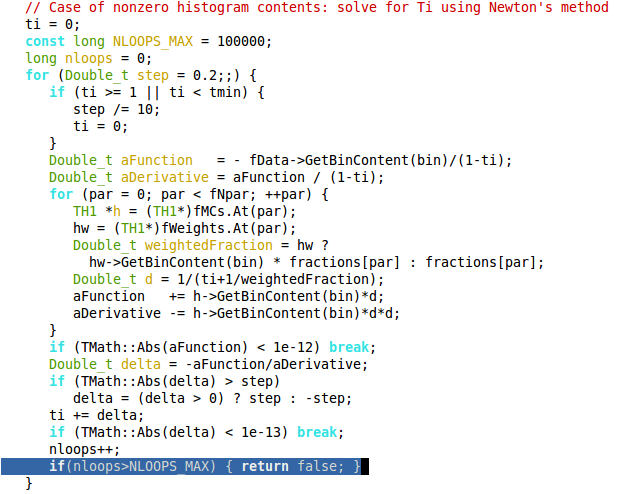
\includegraphics[width=0.8\textwidth]{dates/20121219/figures/pull/code.png}
}



%===========================================
%  Unfolded plots
%===========================================

\section{ Cross-sections }
\slide{ Status }
{
\iteb
\item Added full McAtNlo and PowhegHerwig statistics
\item Added PDF reweighting systematics
\iteb
\item $CT10nlo$
\item $MSTW2008nlo68cl$
\item $HERAPDF15NLO_EIG$
\item $NNPDF23_nlo_as_0118$
\item $abm11_5n_nlo$
\itee
\item Added W pt reweighting systematics
\iteb
\item Nominal is PowhegPythia8
\item Maximum deviation wrt Sherpa14 or PythiaMC10
\itee
\itee
}


\section{ Single-differential POS }
\begin{frame}{$\Wplus \rightarrow \mu^+ \nu$}
 \begin{center}
   \includegraphics[width=0.6\textwidth]<1>{dates/20121219/figures/xsec/POS/Wmn_Unf_proj.pdf}
   \includegraphics[width=0.6\textwidth]<2>{dates/20121219/figures/xsec/POS/Wmn_unf2010_proj.pdf}
   \includegraphics[width=0.6\textwidth]<3>{dates/20121219/figures/xsec/POS/Wmn_Unc_proj.pdf}
 \end{center}
\end{frame}

\section{ Single-differential NEG }
\begin{frame}{$\Wminus \rightarrow \mu^- \nu$}
 \begin{center}
   \includegraphics[width=0.6\textwidth]<1>{dates/20121219/figures/xsec/NEG/Wmn_Unf_proj.pdf}
   \includegraphics[width=0.6\textwidth]<2>{dates/20121219/figures/xsec/NEG/Wmn_unf2010_proj.pdf}
   \includegraphics[width=0.6\textwidth]<3>{dates/20121219/figures/xsec/NEG/Wmn_Unc_proj.pdf}
 \end{center}
\end{frame}


\section{ Double-differential POS}

\begin{frame}{Unfolded cross-sections: $\Wplus \rightarrow \mu^+ \nu$}
 \begin{center}
   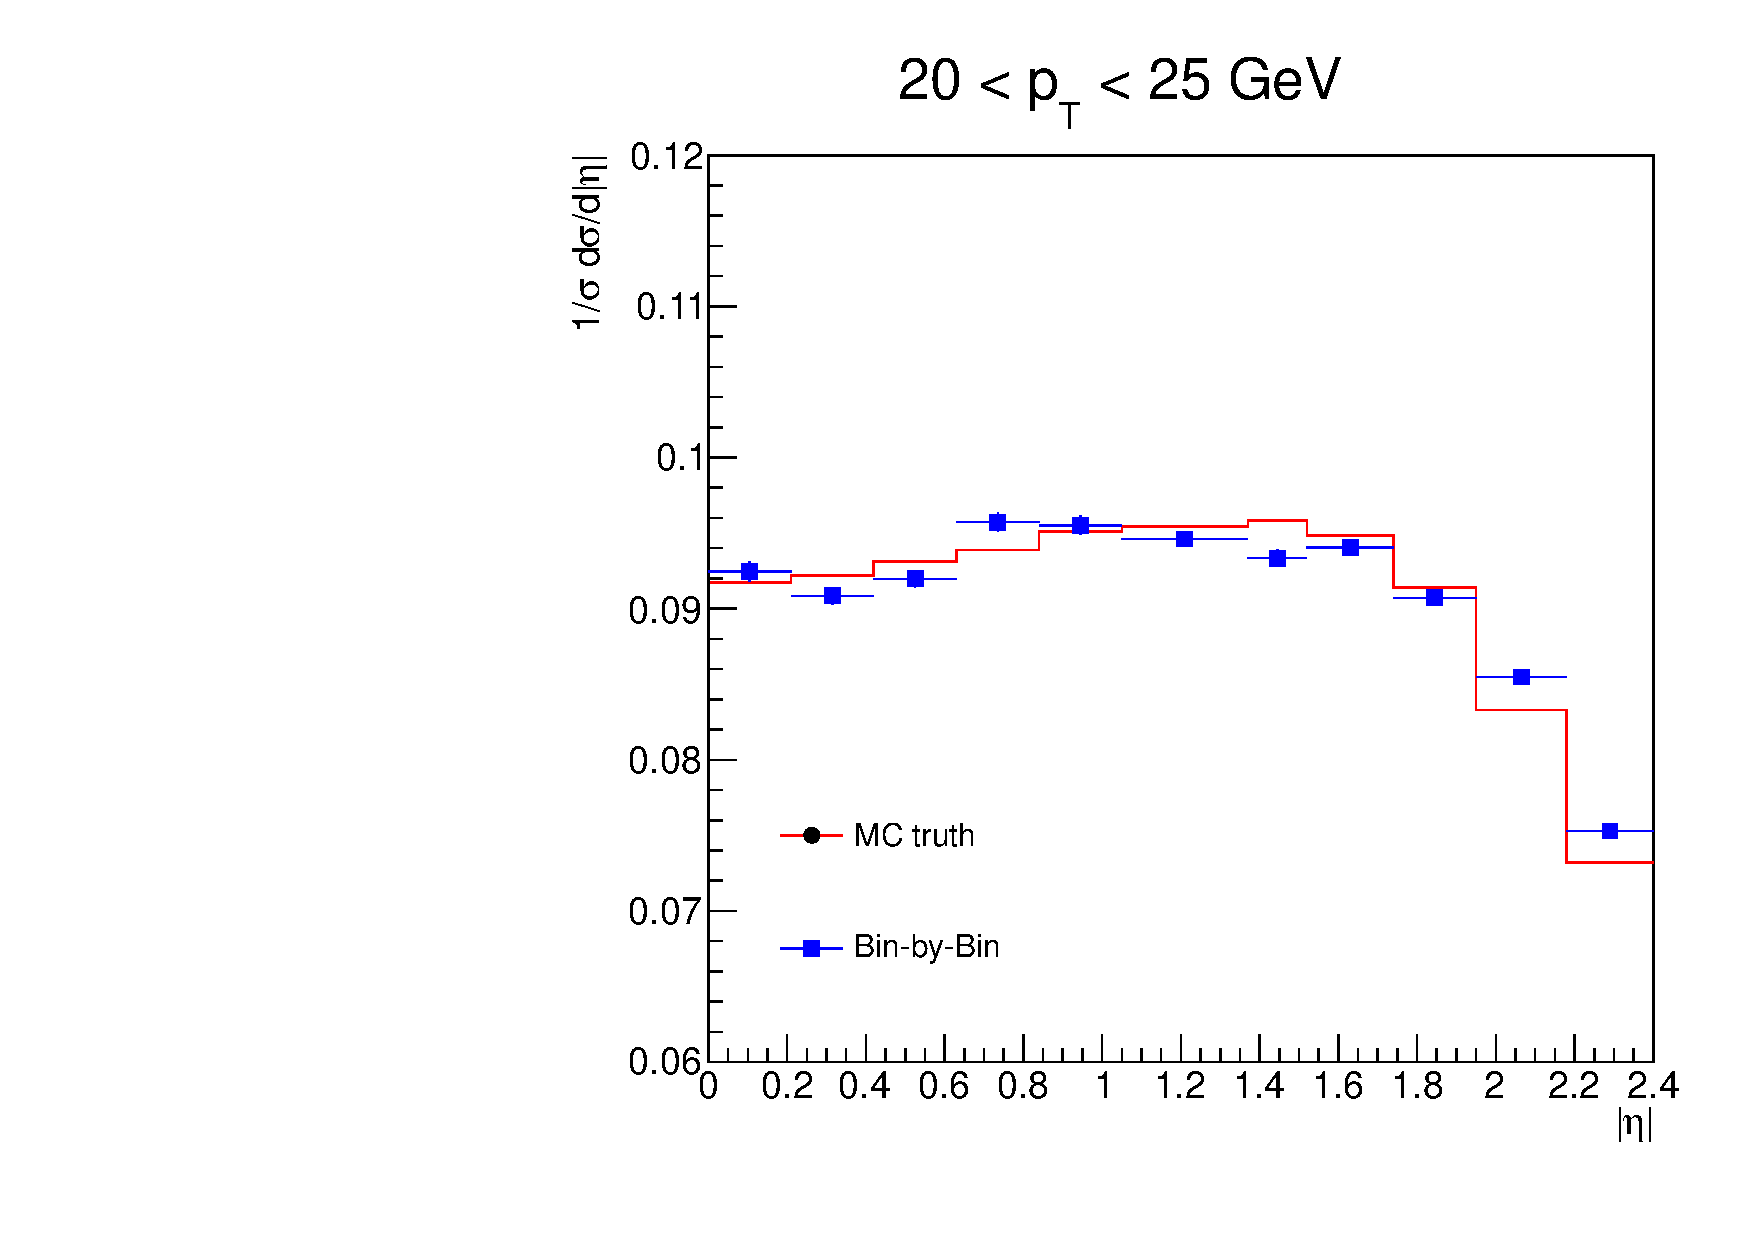
\includegraphics[width=0.6\textwidth]{dates/20121219/figures/xsec/POS/Wmn_Unf_2d_Slice_1.pdf}
 \end{center}
\end{frame}

\begin{frame}{Unfolded cross-sections: $\Wplus \rightarrow \mu^+ \nu$}
 \begin{center}
   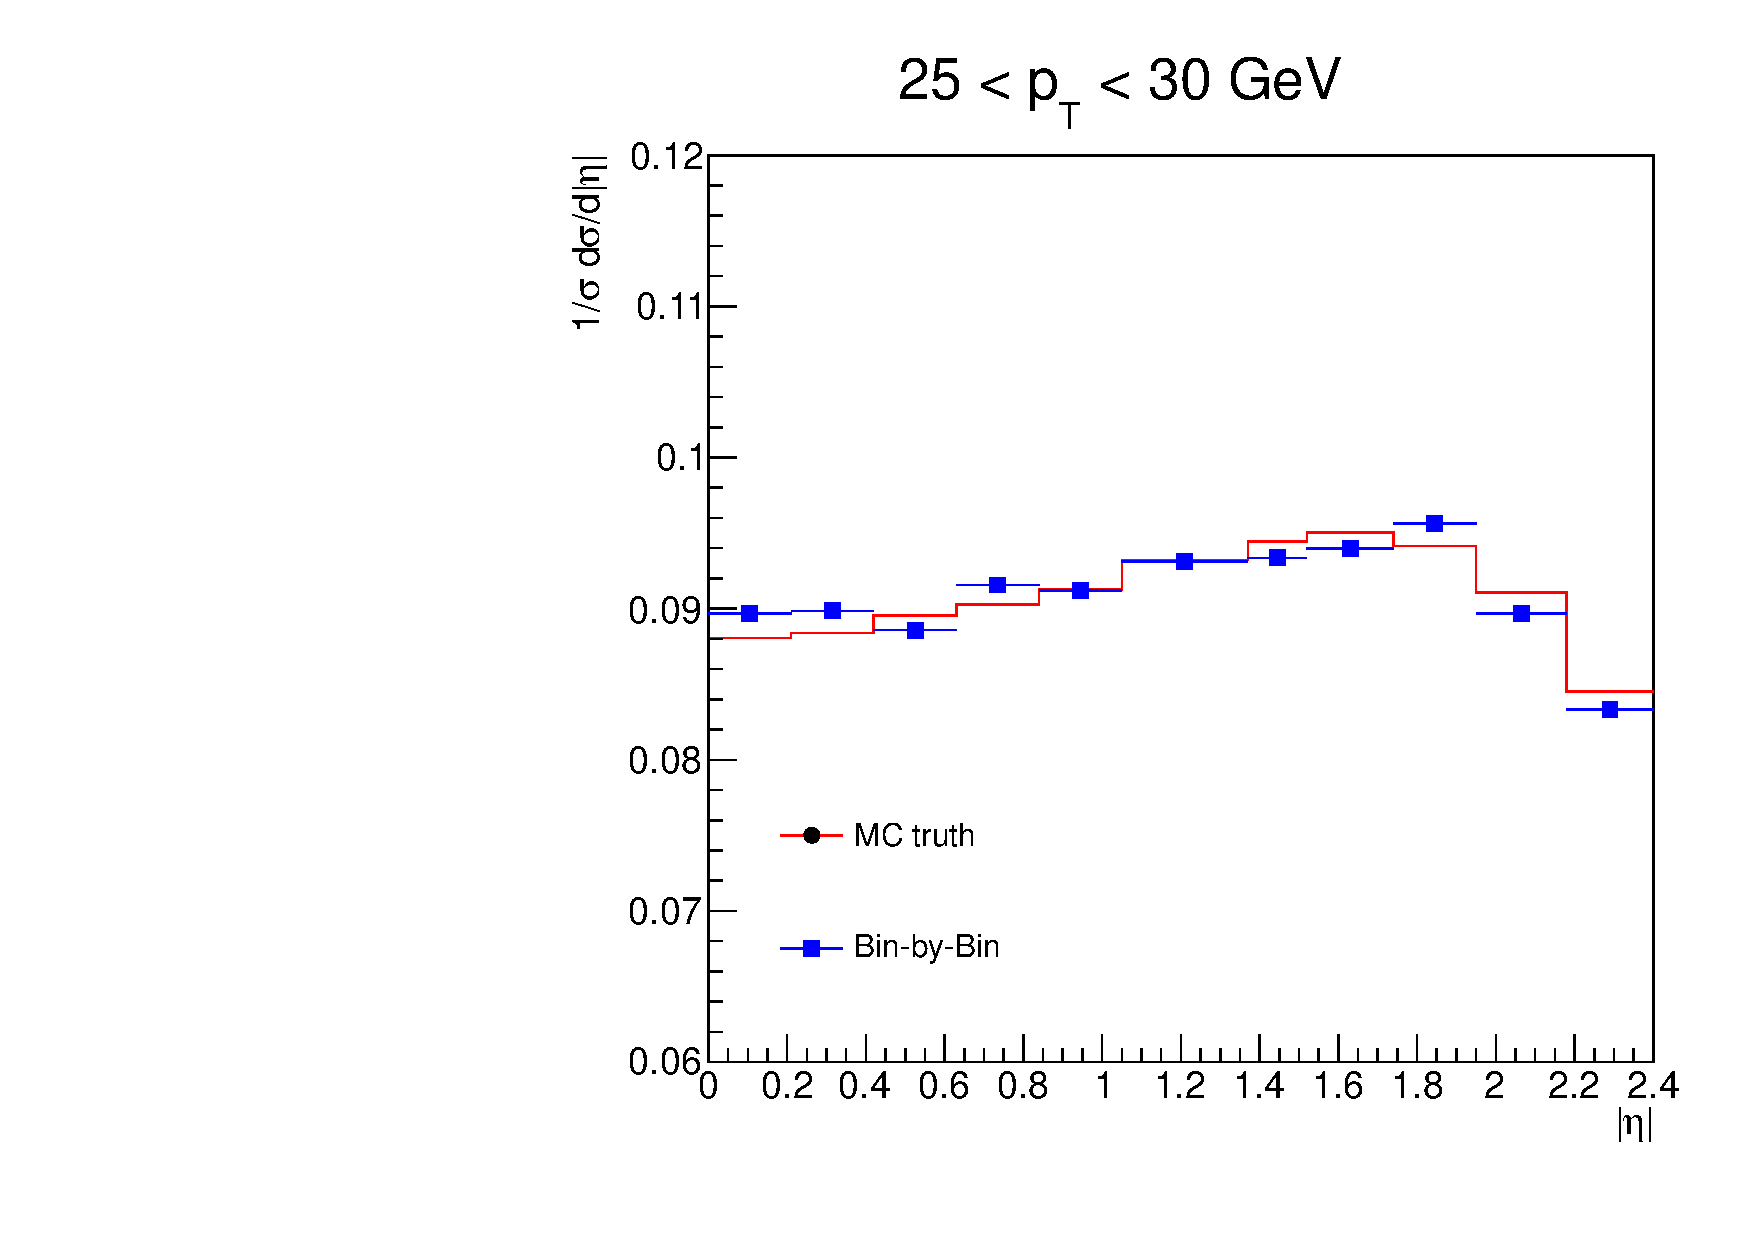
\includegraphics[width=0.3\textwidth]{dates/20121219/figures/xsec/POS/Wmn_Unf_2d_Slice_2.pdf}
   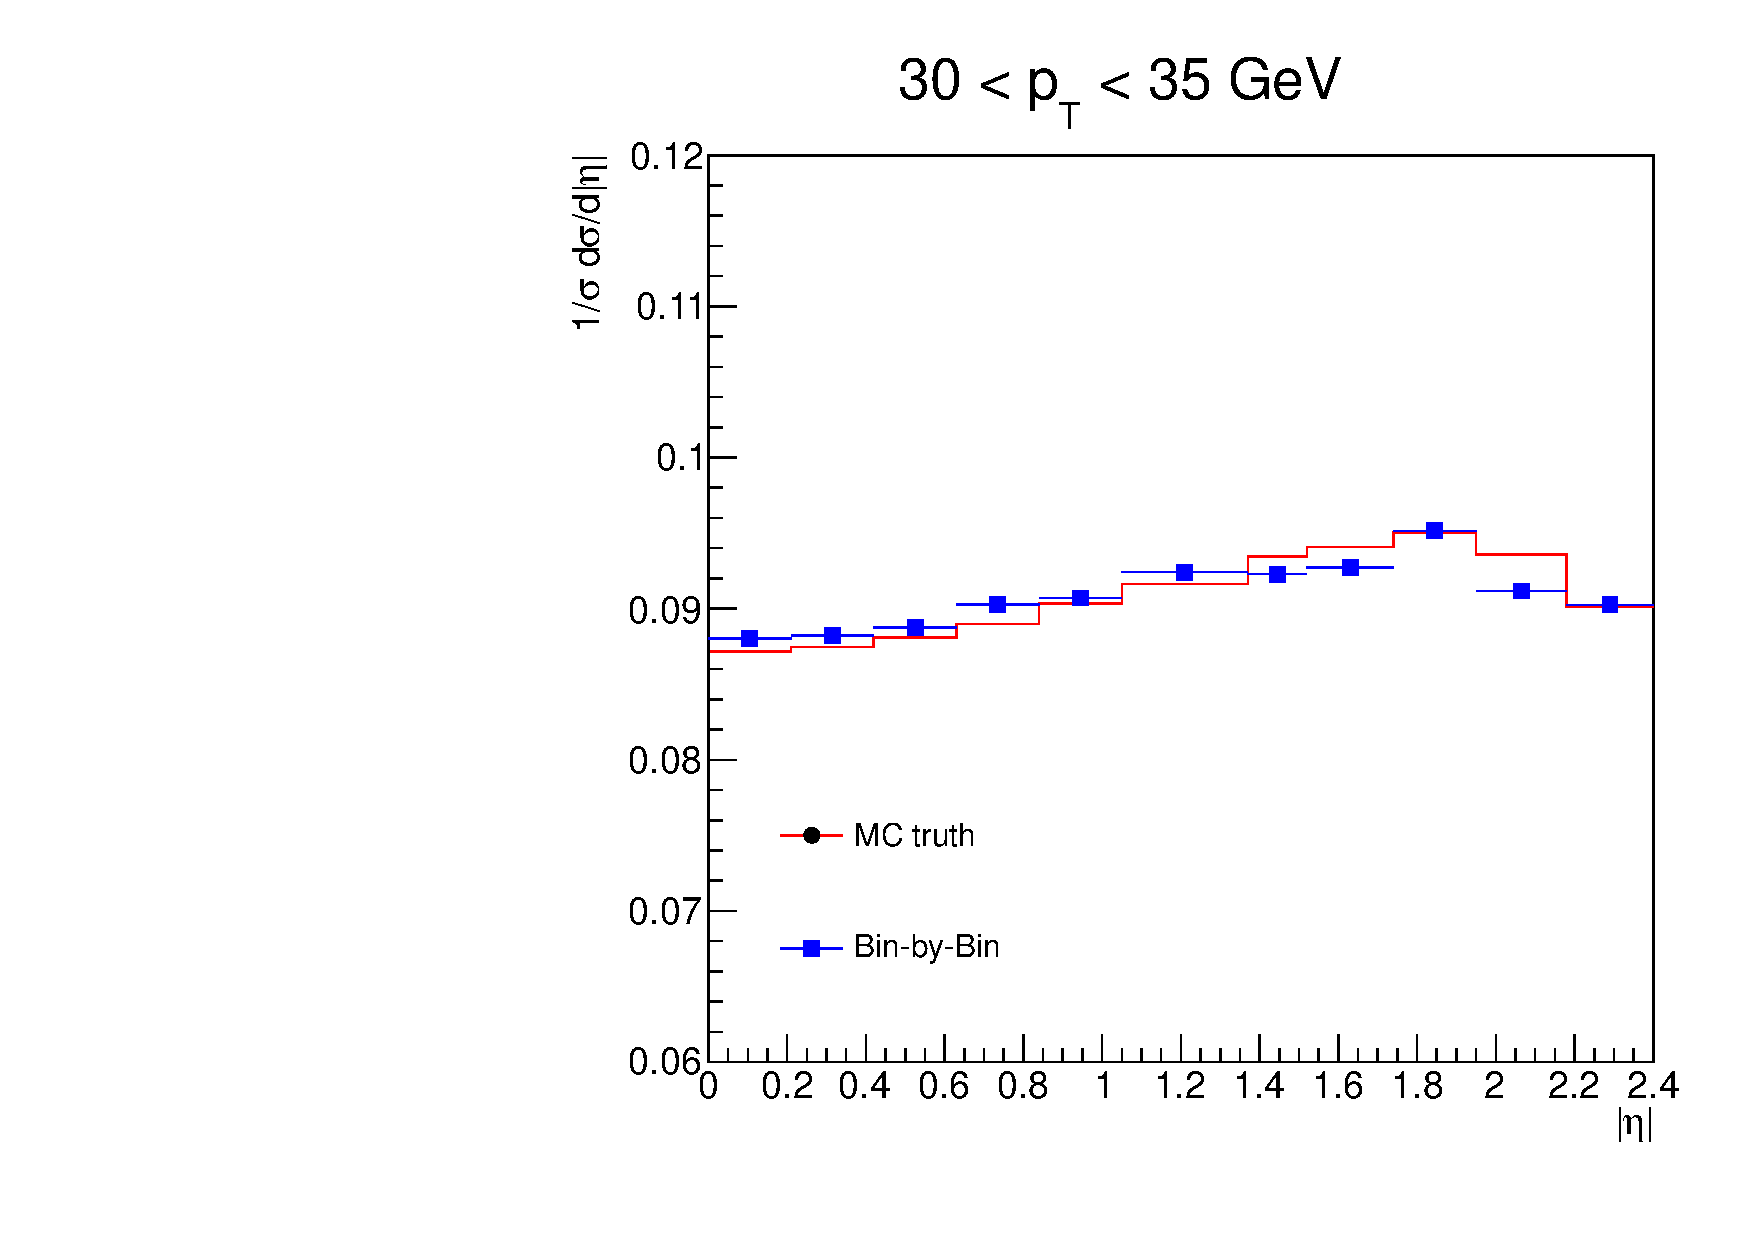
\includegraphics[width=0.3\textwidth]{dates/20121219/figures/xsec/POS/Wmn_Unf_2d_Slice_3.pdf}
   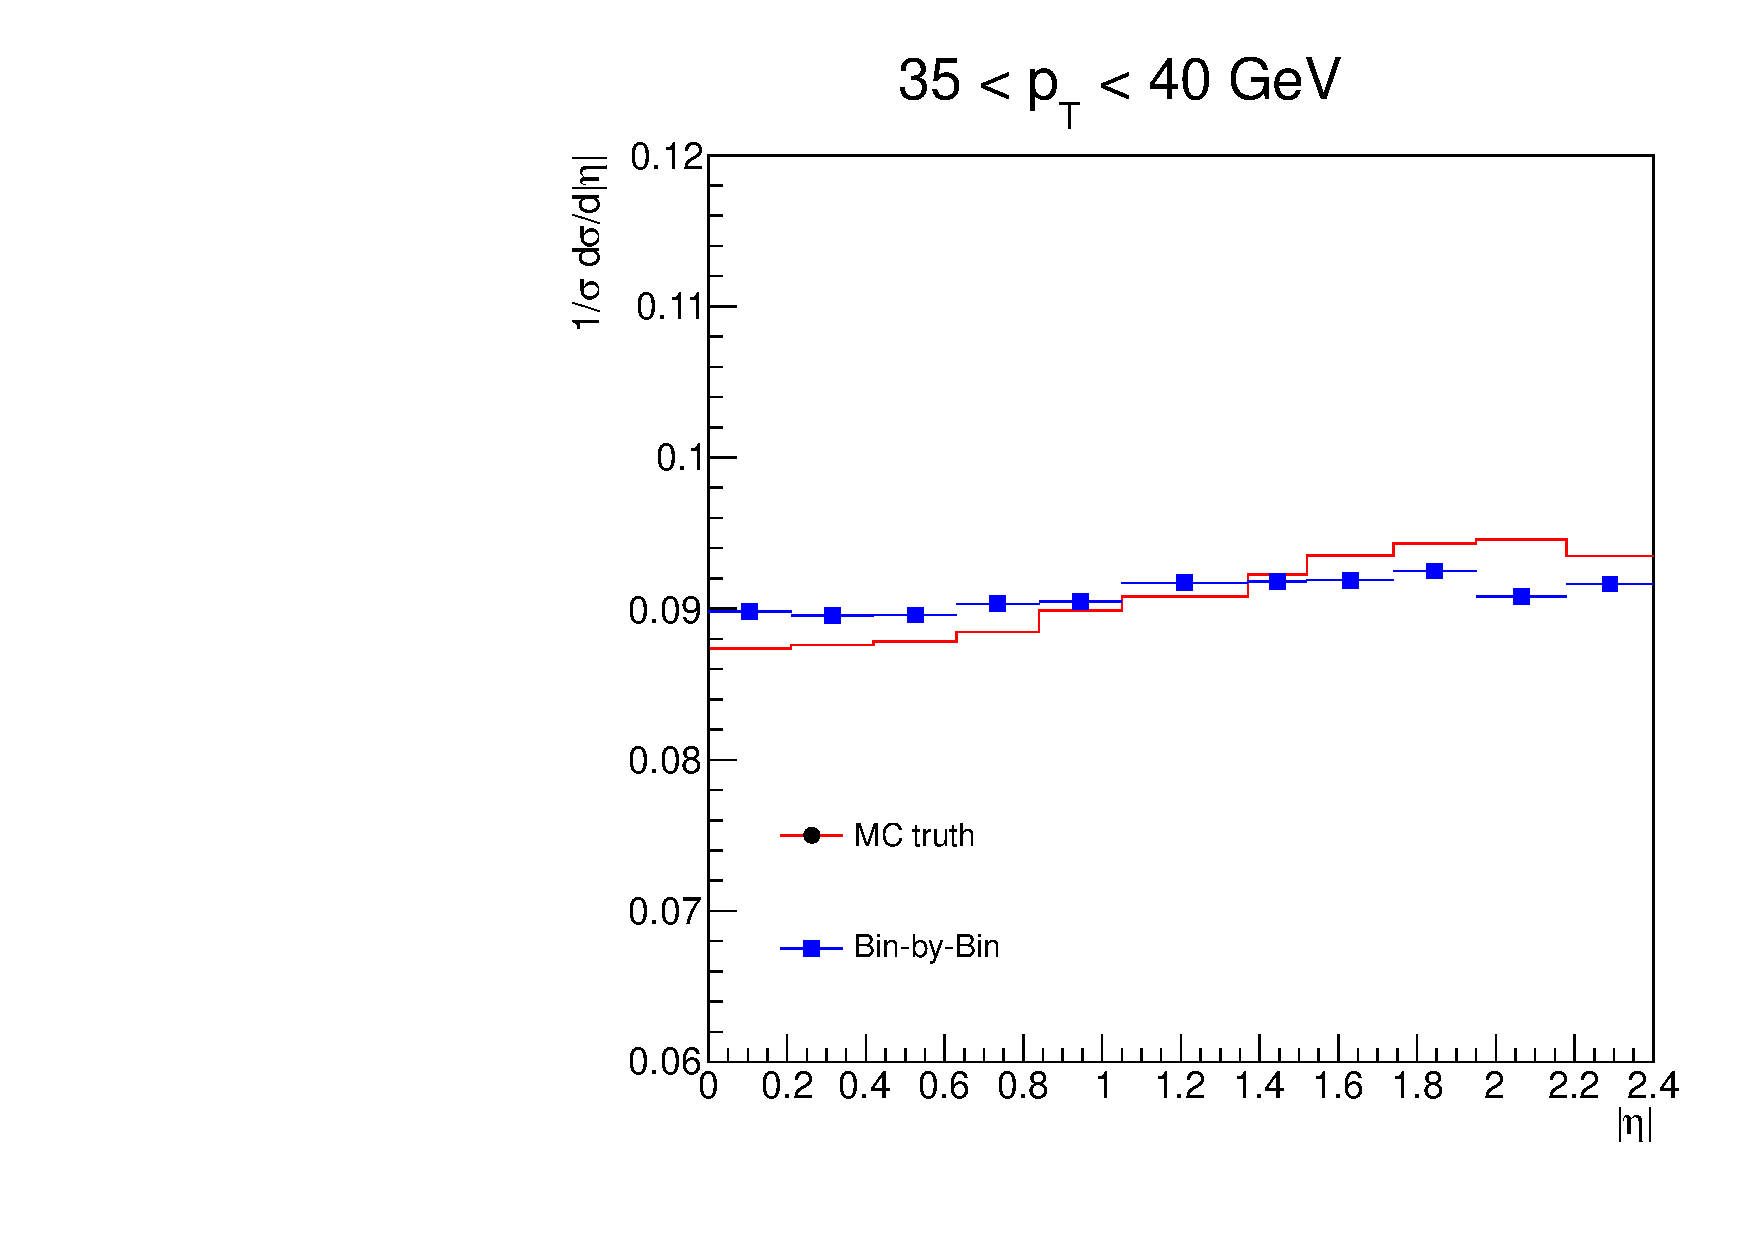
\includegraphics[width=0.3\textwidth]{dates/20121219/figures/xsec/POS/Wmn_Unf_2d_Slice_4.pdf}
 \end{center}
 \begin{center}
   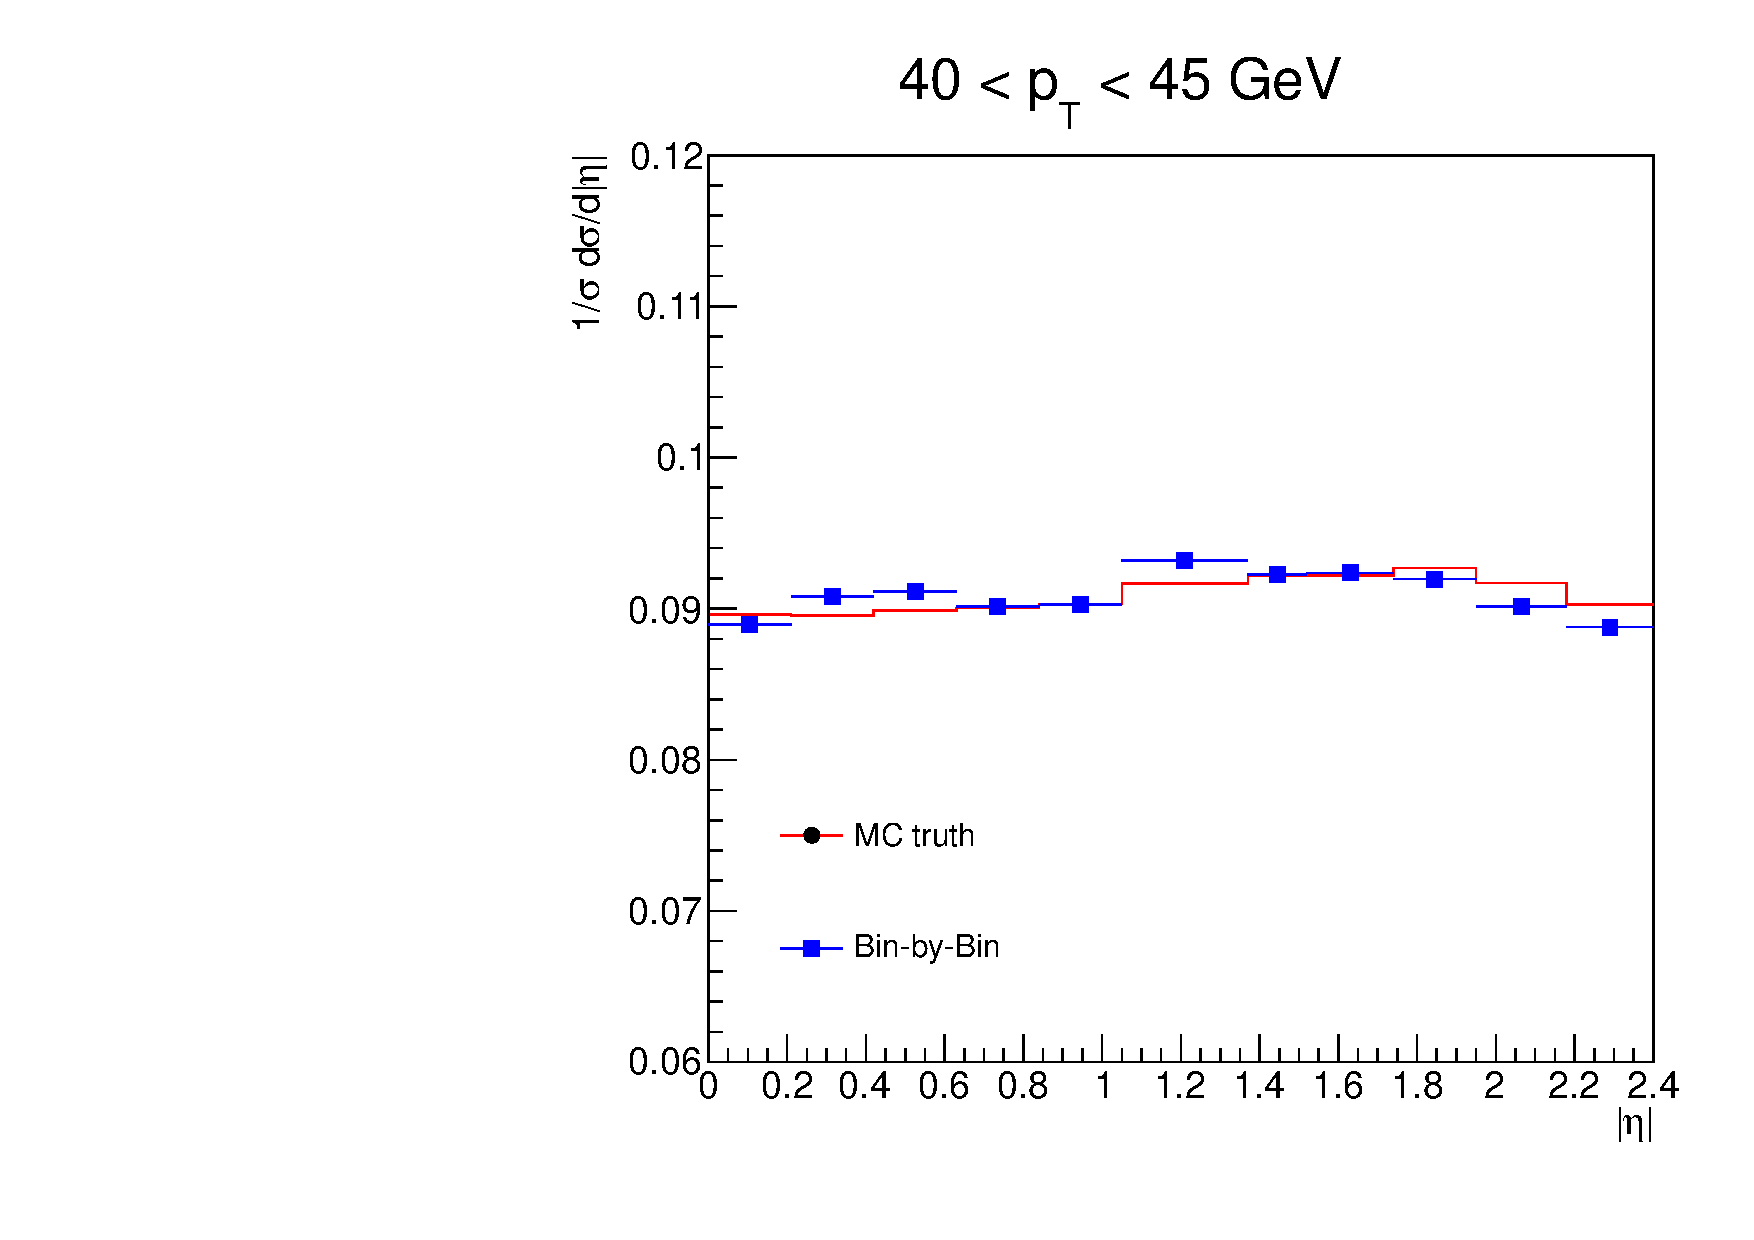
\includegraphics[width=0.3\textwidth]{dates/20121219/figures/xsec/POS/Wmn_Unf_2d_Slice_5.pdf}
   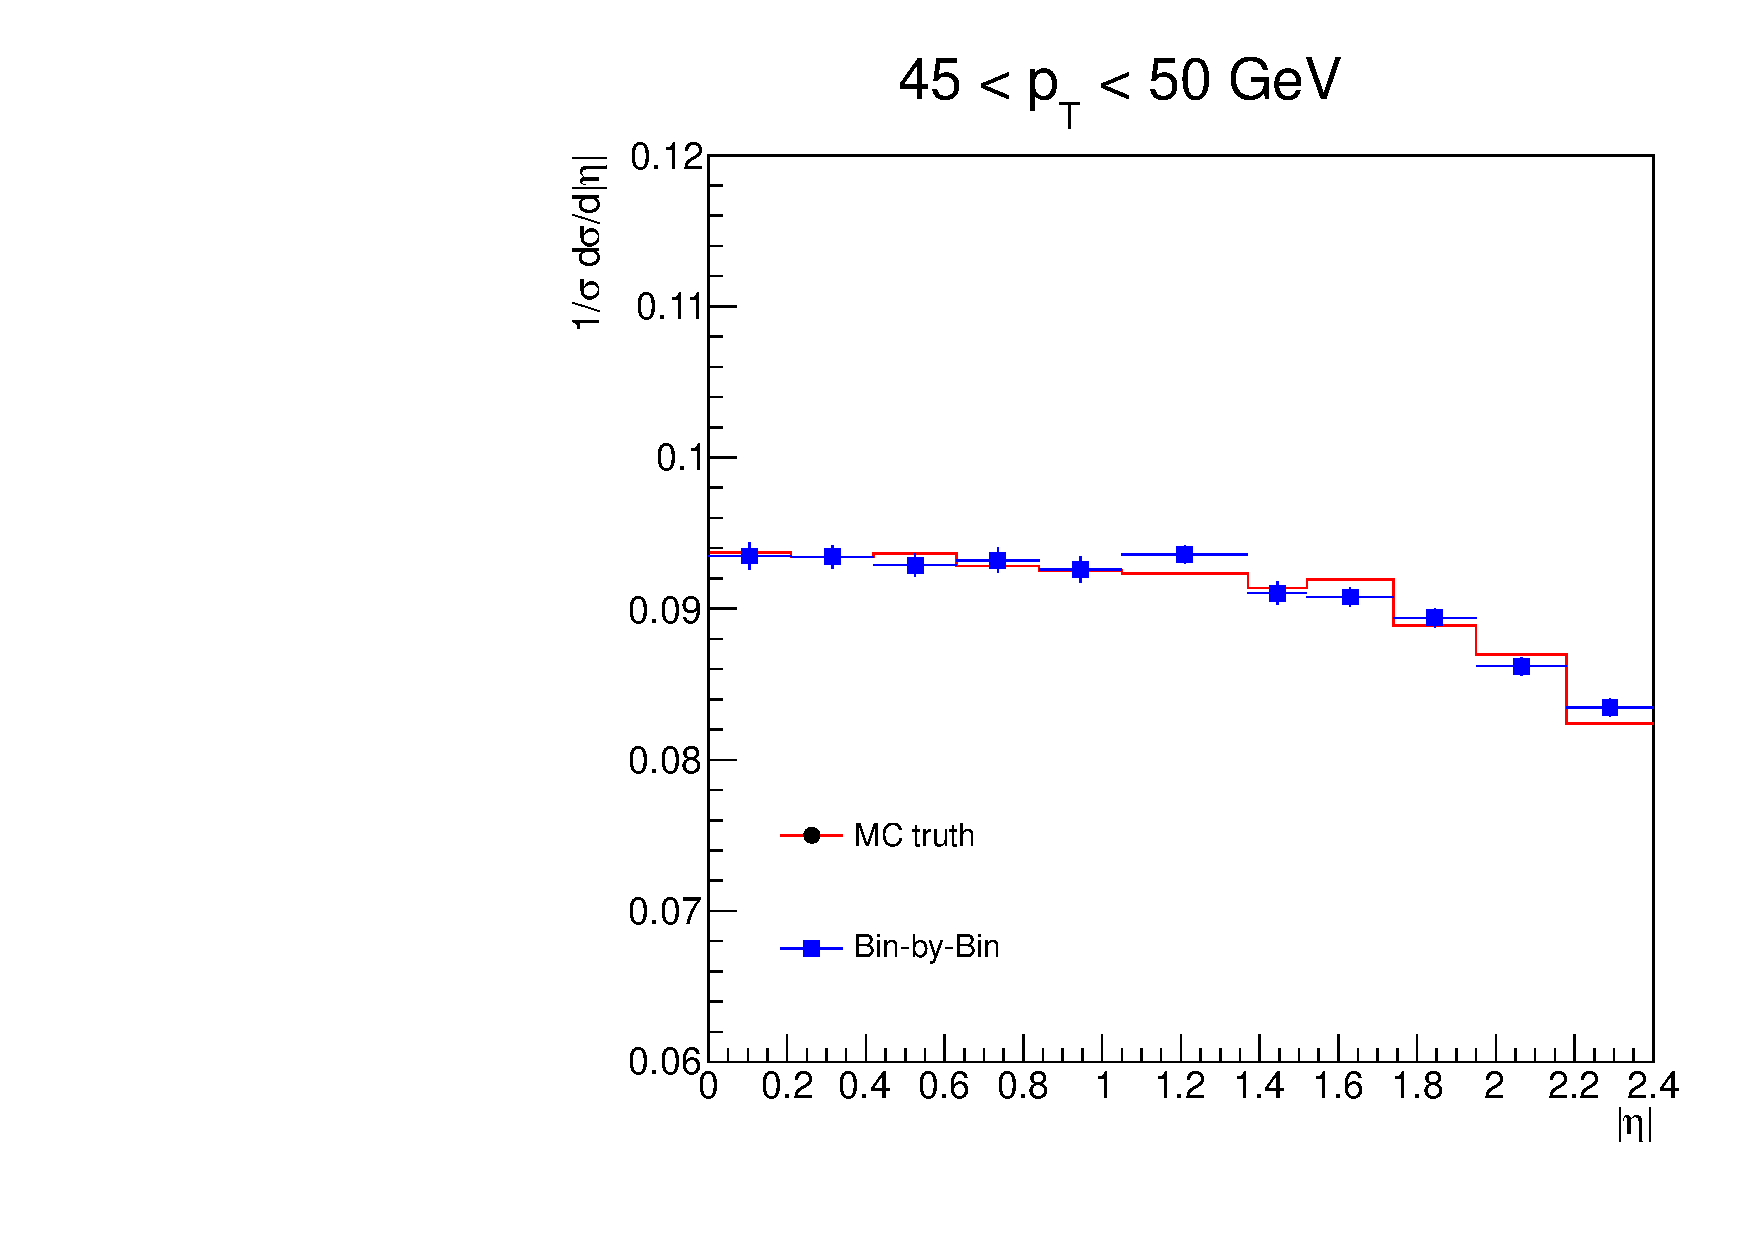
\includegraphics[width=0.3\textwidth]{dates/20121219/figures/xsec/POS/Wmn_Unf_2d_Slice_6.pdf}
   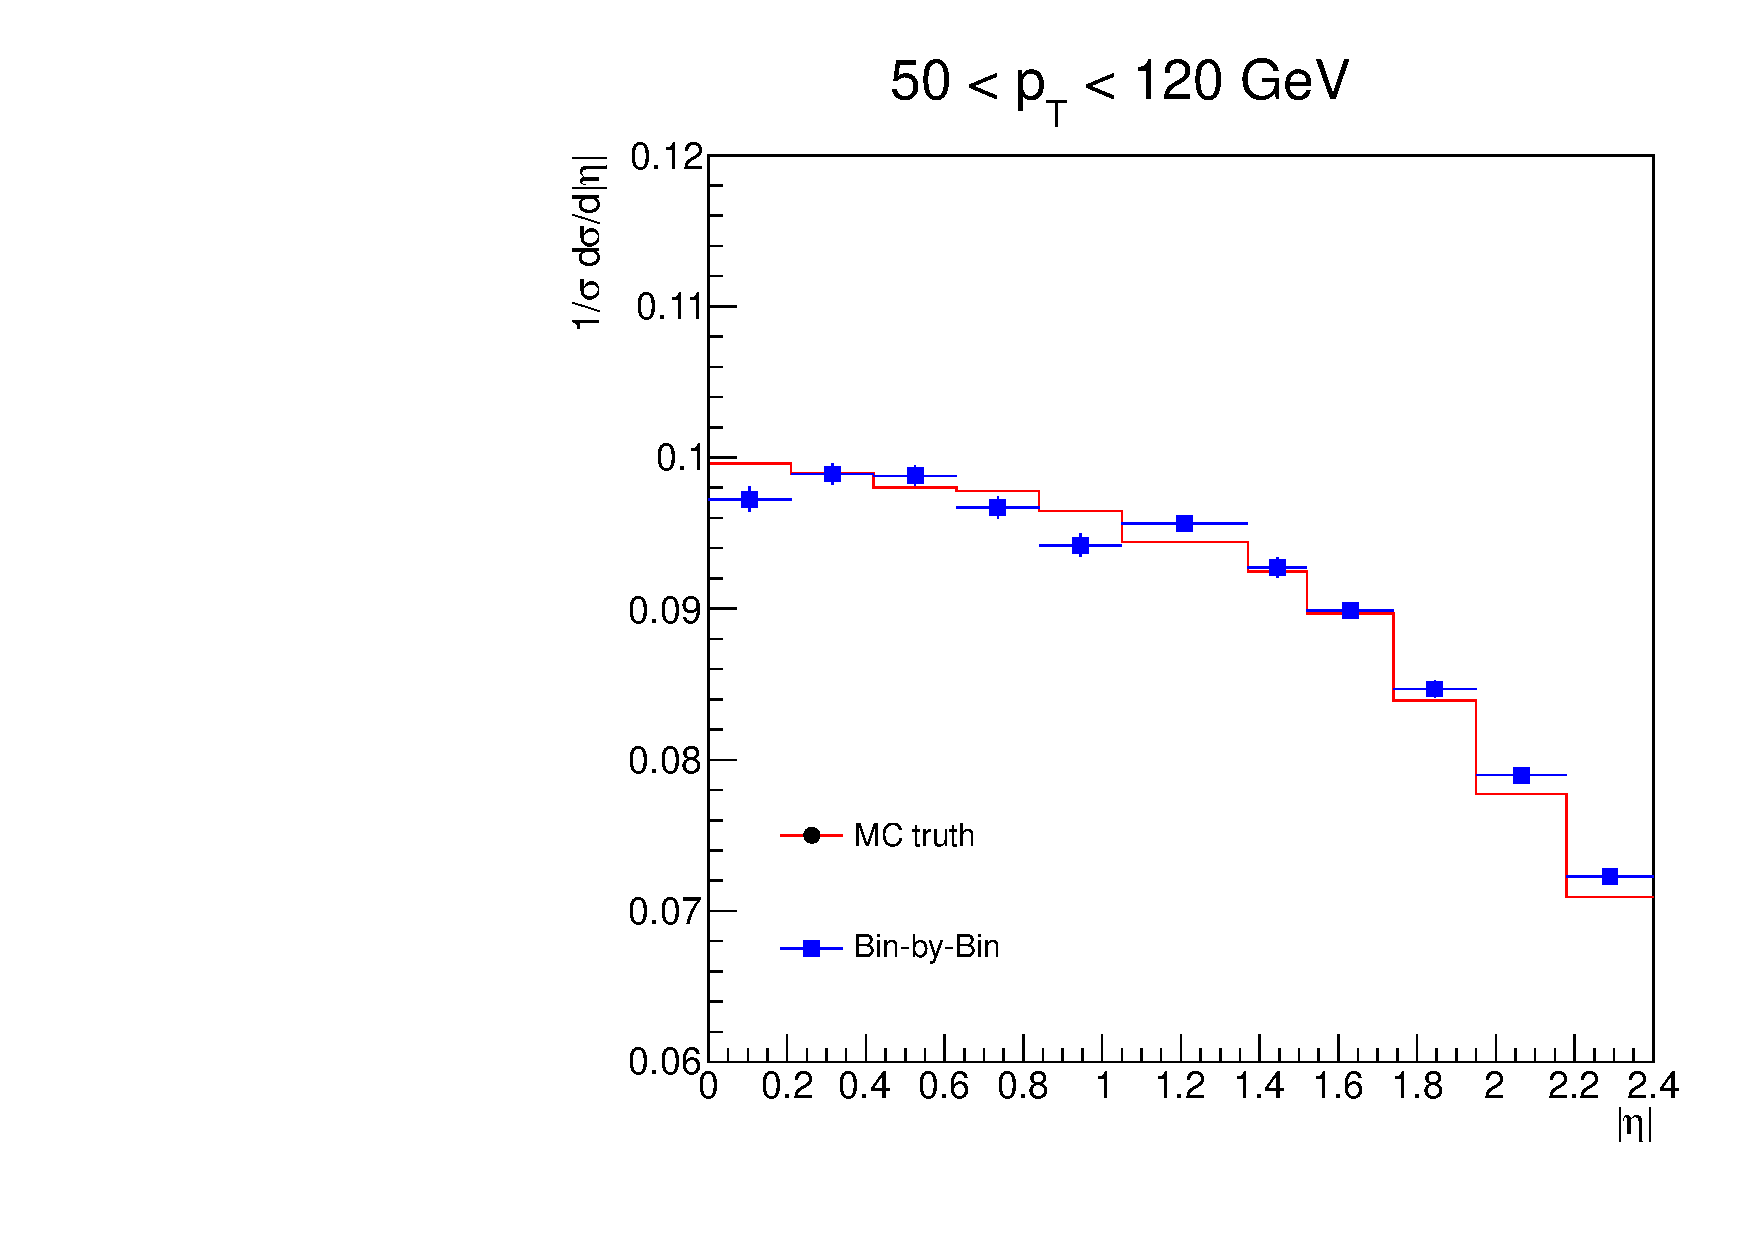
\includegraphics[width=0.3\textwidth]{dates/20121219/figures/xsec/POS/Wmn_Unf_2d_Slice_7.pdf}
 \end{center}
\end{frame}


\begin{frame}{Systematic Uncertainties: $\Wplus \rightarrow \mu^+ \nu$}
 \begin{center}
   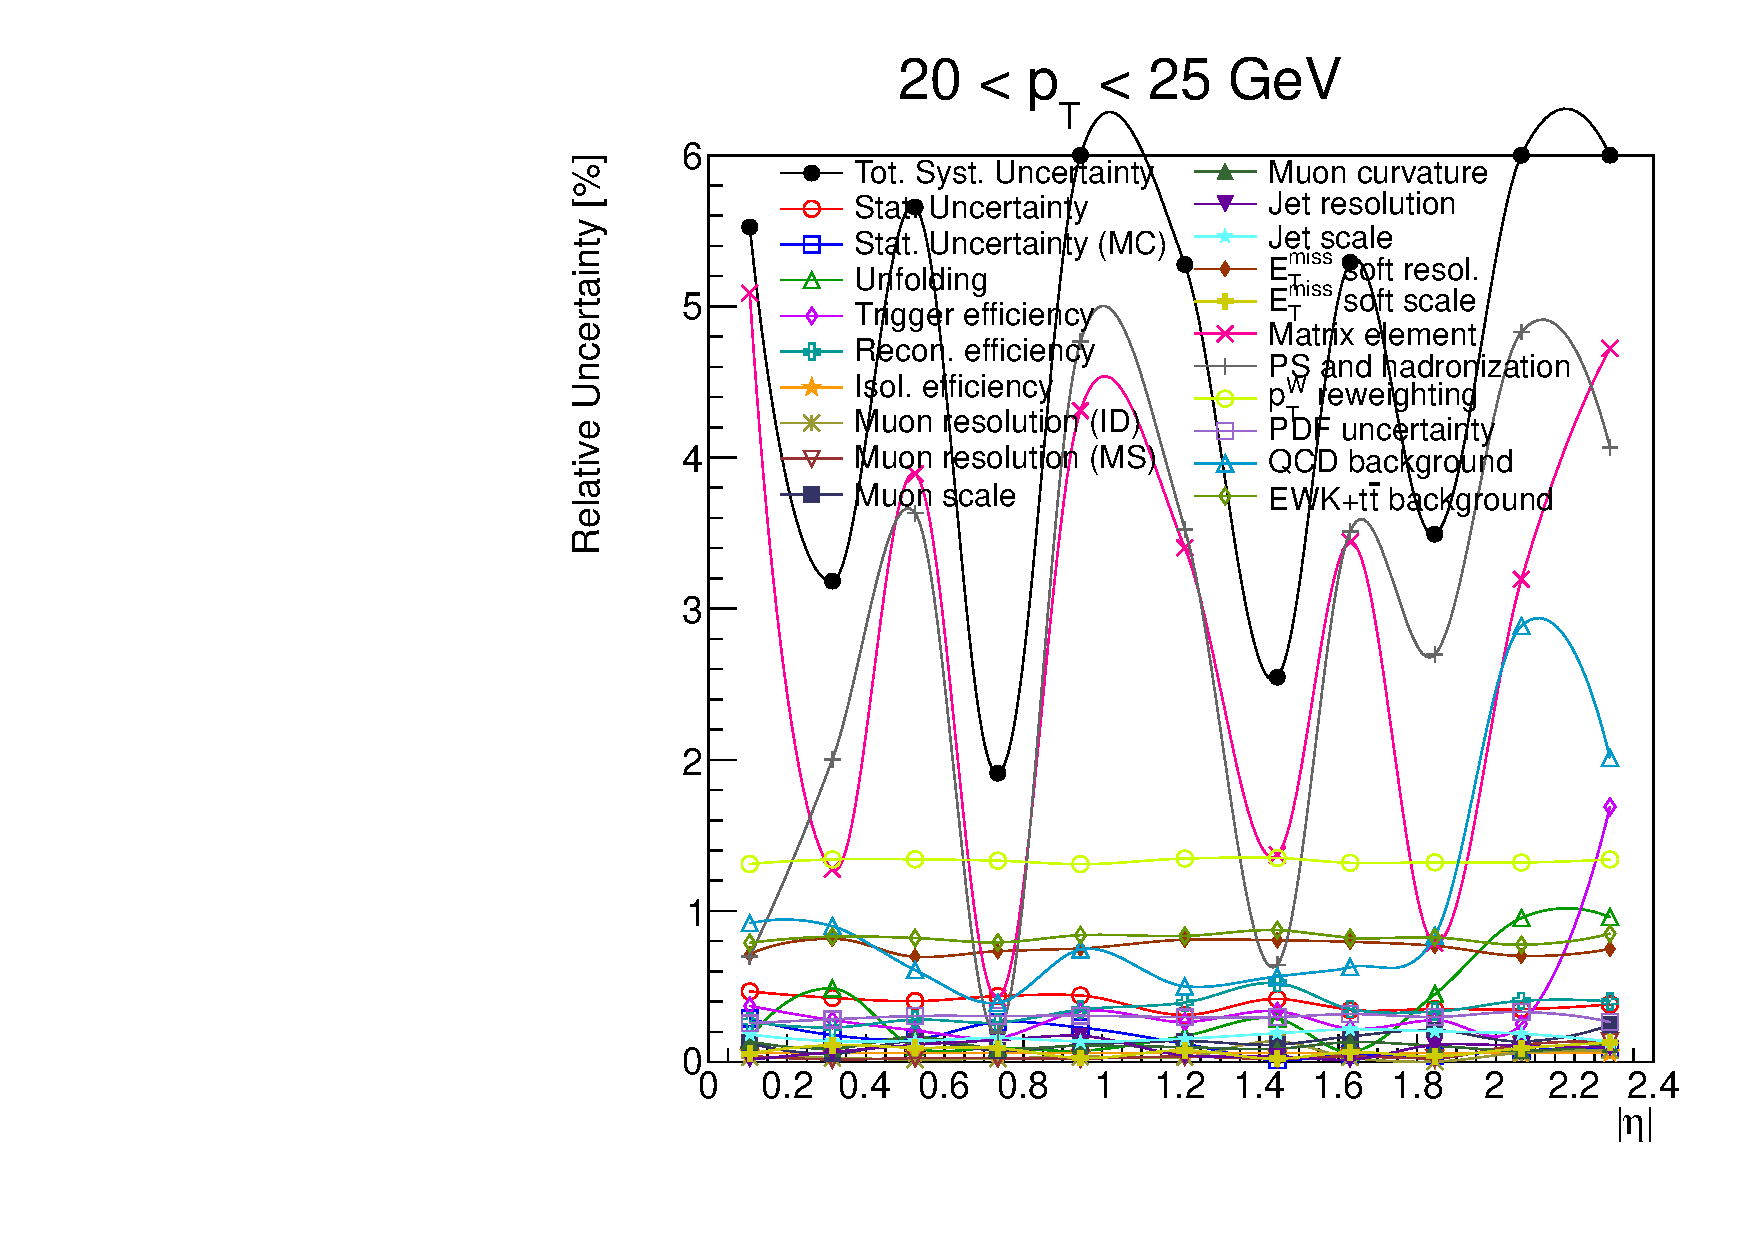
\includegraphics[width=0.6\textwidth]{dates/20121219/figures/xsec/POS/Wmn_Unc_2d_Slice_1.pdf}
 \end{center}
\end{frame}

\begin{frame}{Systematic Uncertainties: $\Wplus \rightarrow \mu^+ \nu$}
 \begin{center}
   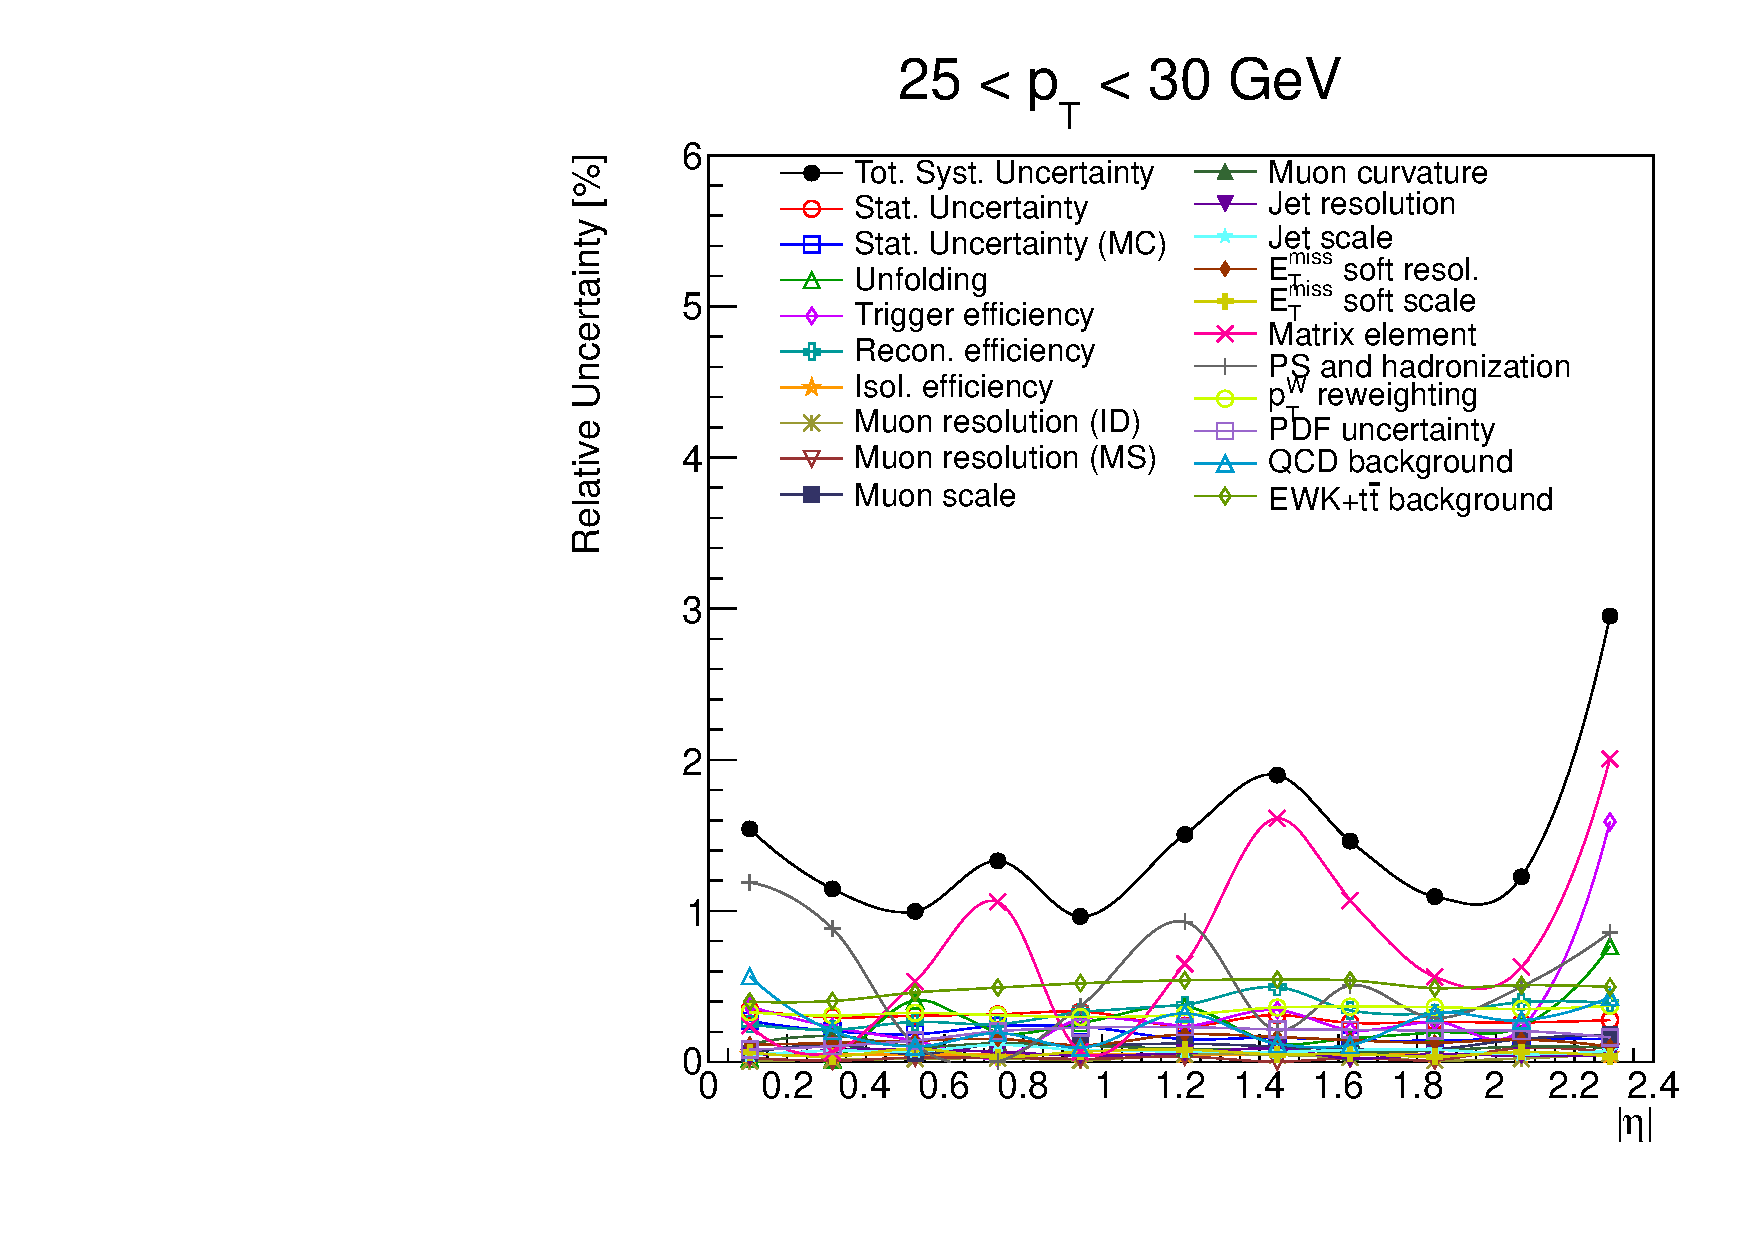
\includegraphics[width=0.3\textwidth]{dates/20121219/figures/xsec/POS/Wmn_Unc_2d_Slice_2.pdf}
   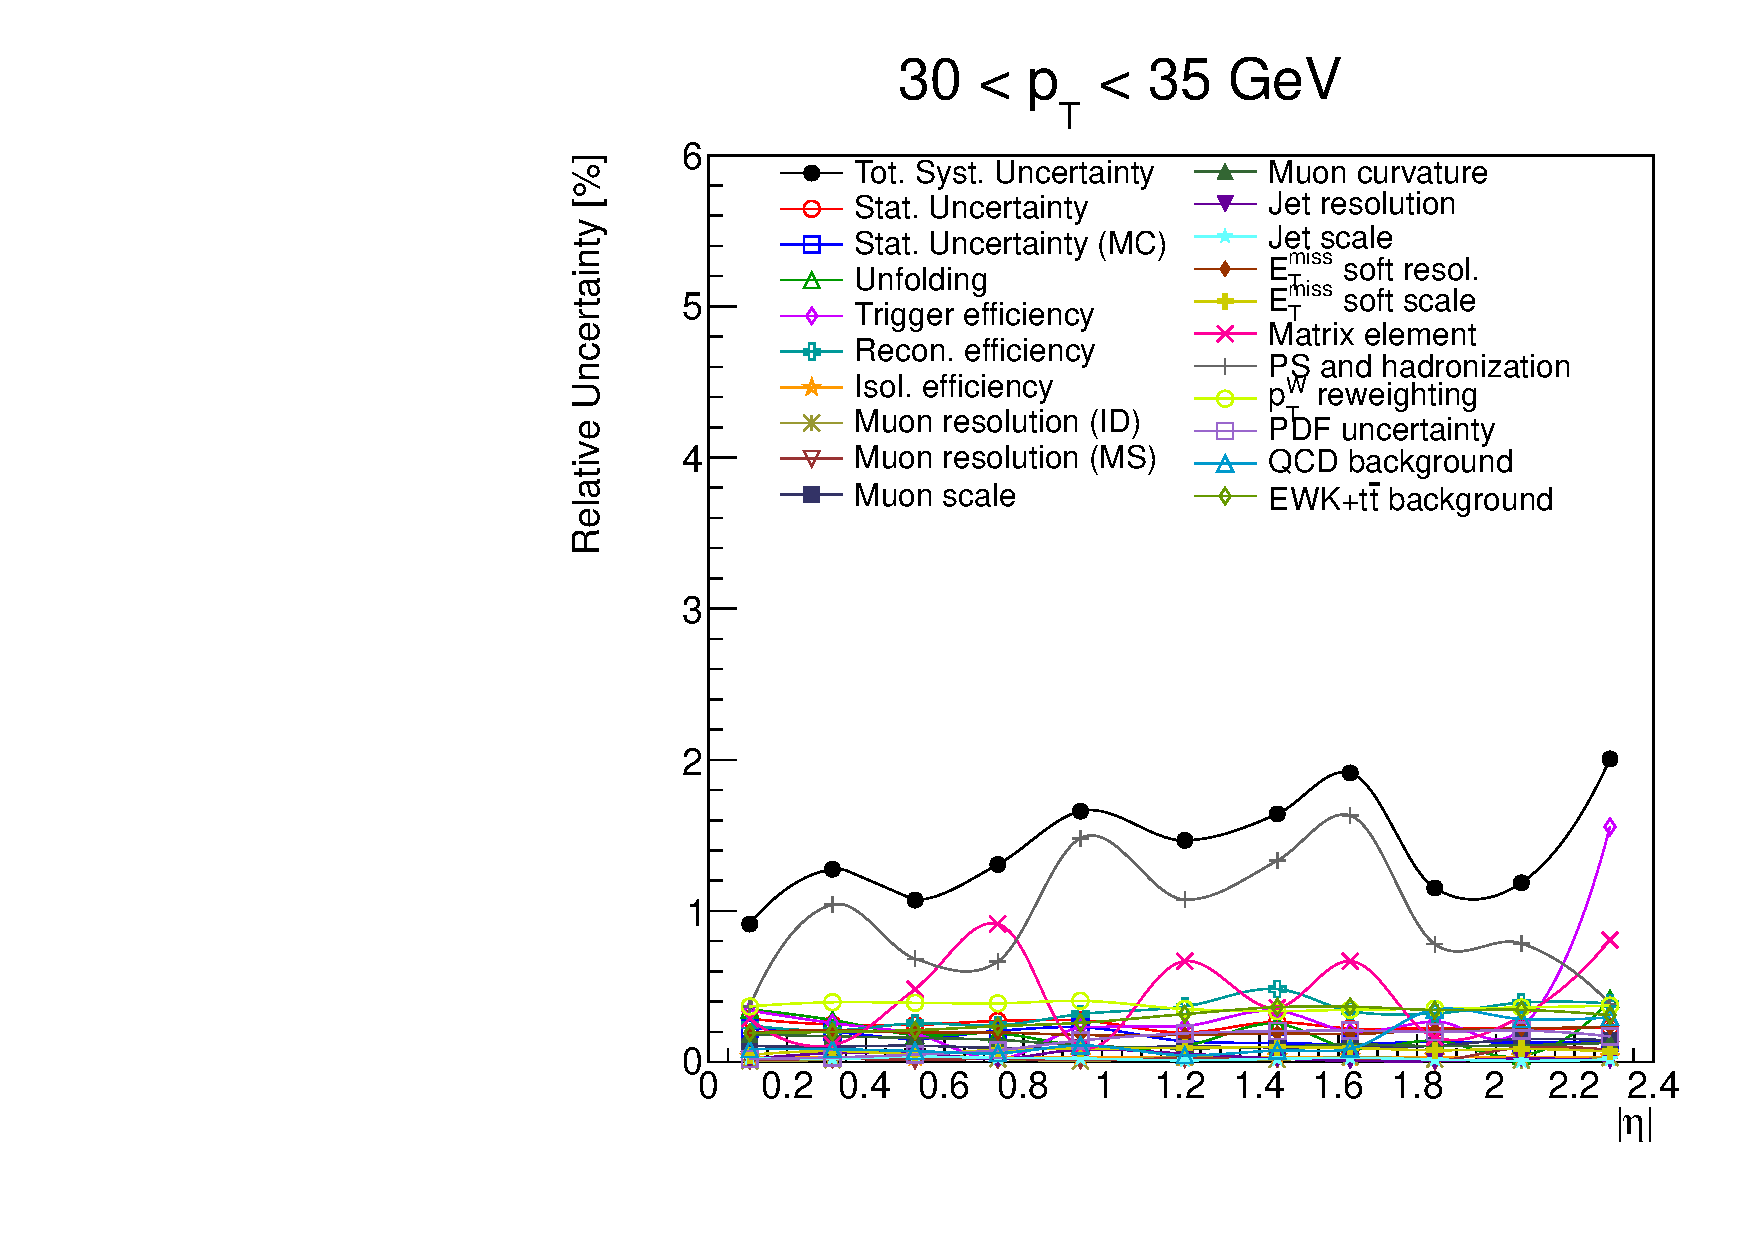
\includegraphics[width=0.3\textwidth]{dates/20121219/figures/xsec/POS/Wmn_Unc_2d_Slice_3.pdf}
   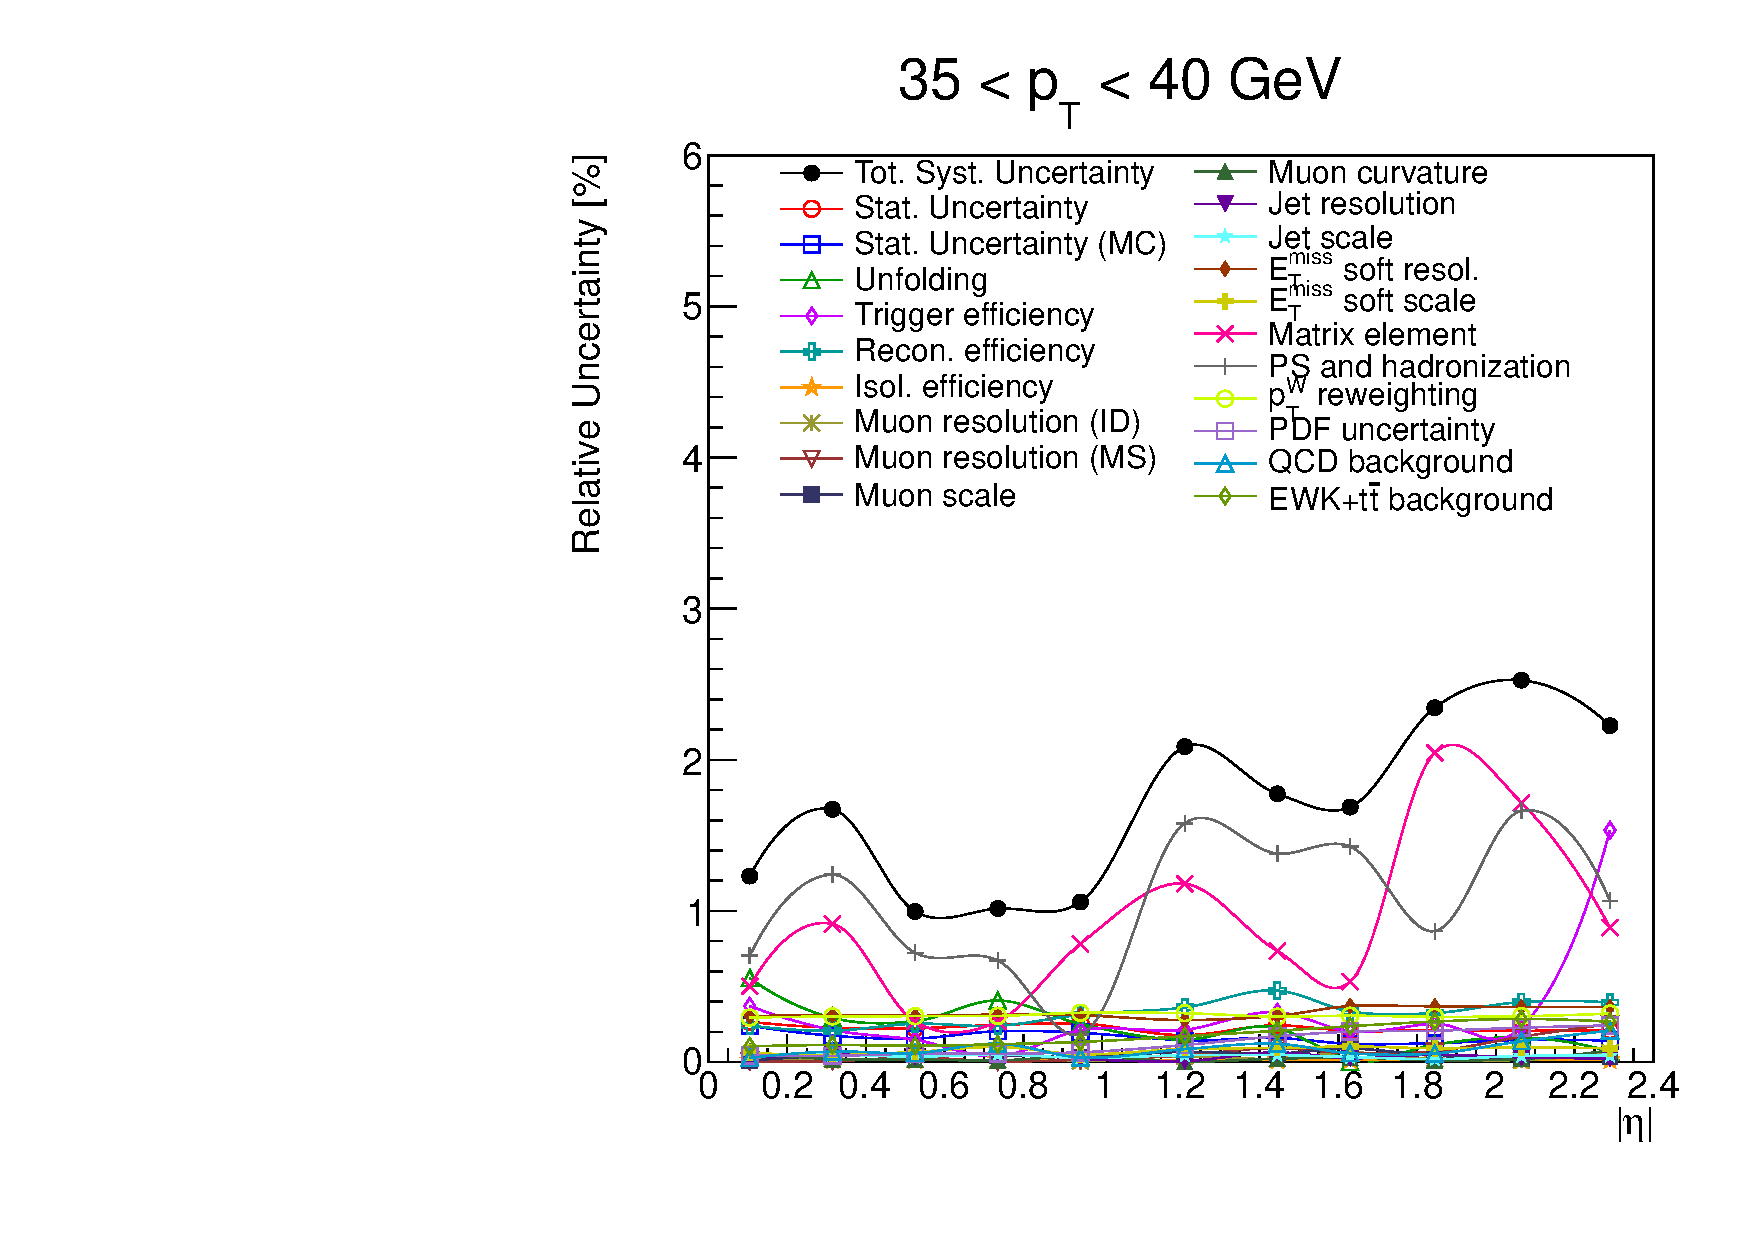
\includegraphics[width=0.3\textwidth]{dates/20121219/figures/xsec/POS/Wmn_Unc_2d_Slice_4.pdf}
 \end{center}
 \begin{center}
   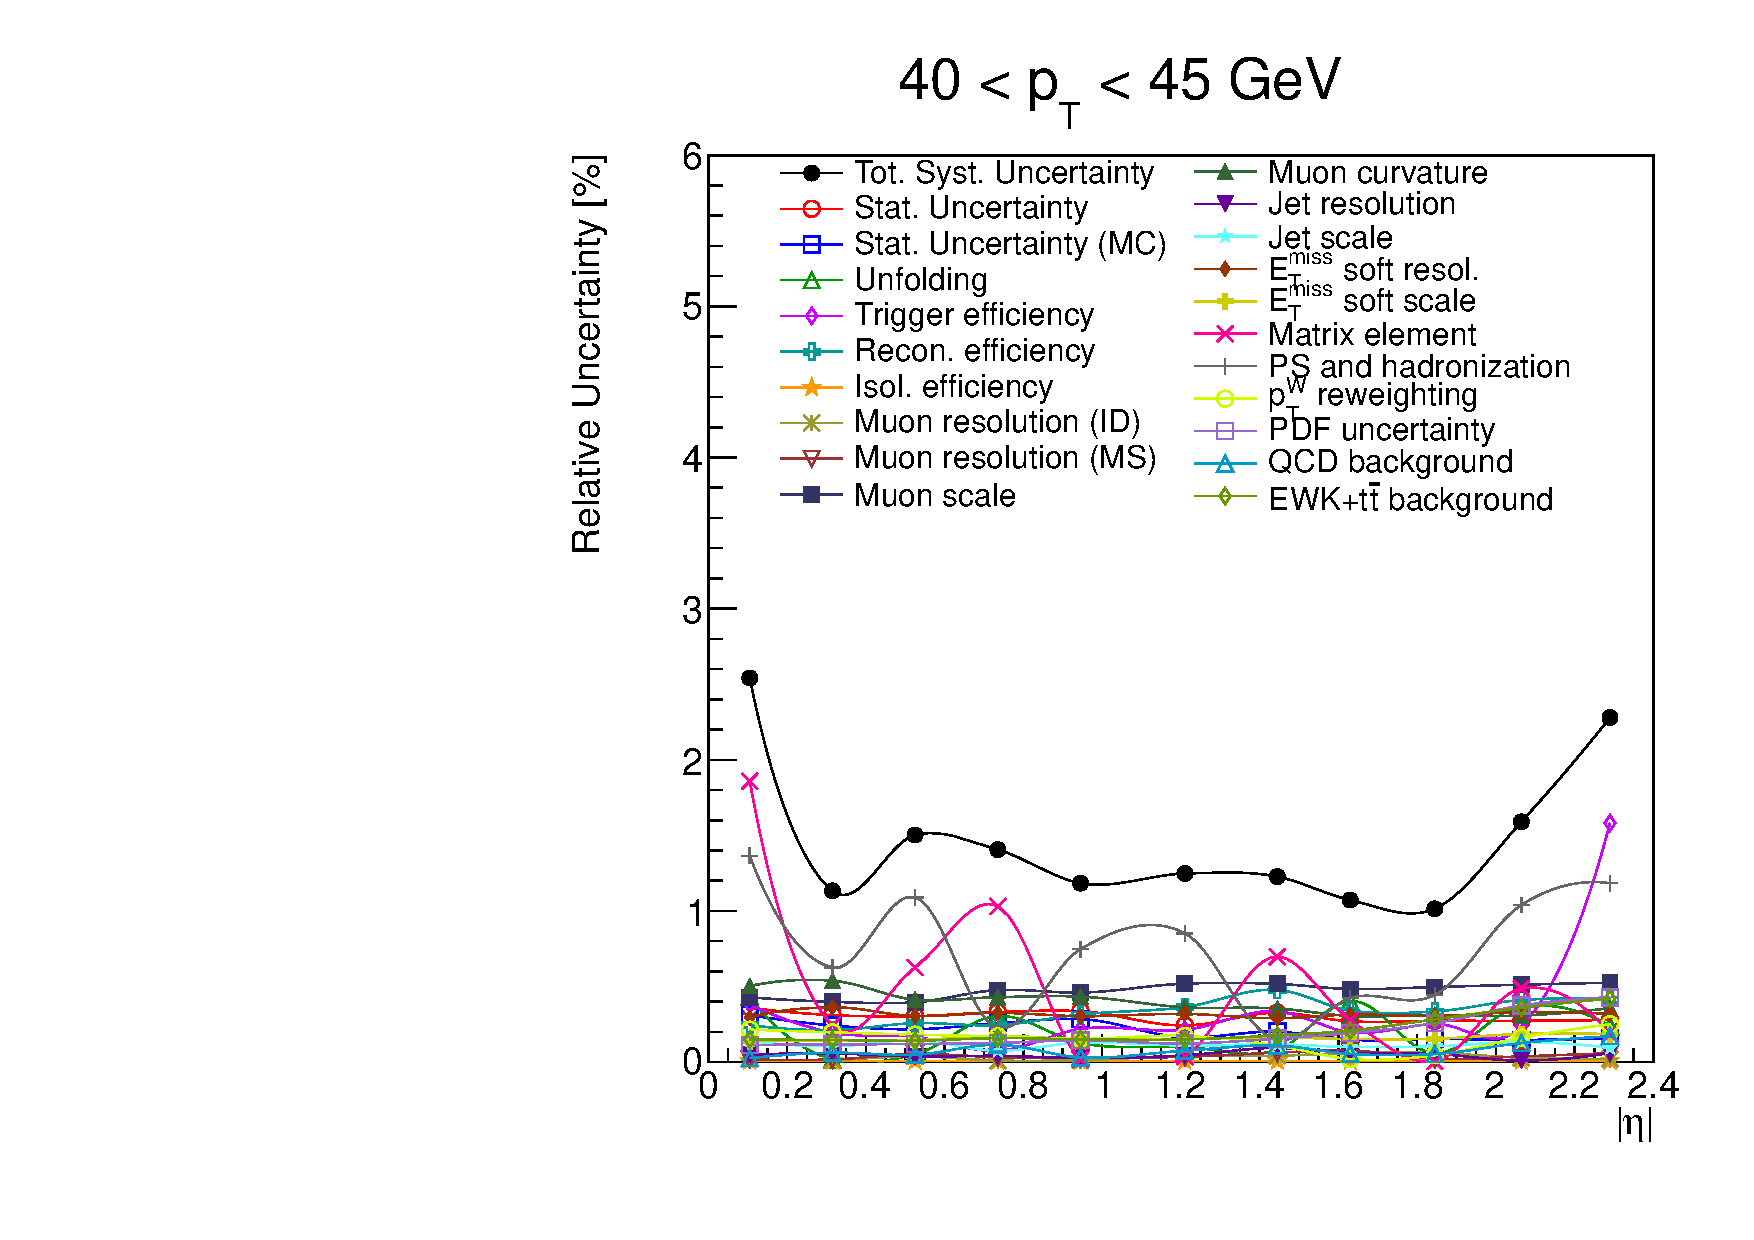
\includegraphics[width=0.3\textwidth]{dates/20121219/figures/xsec/POS/Wmn_Unc_2d_Slice_5.pdf}
   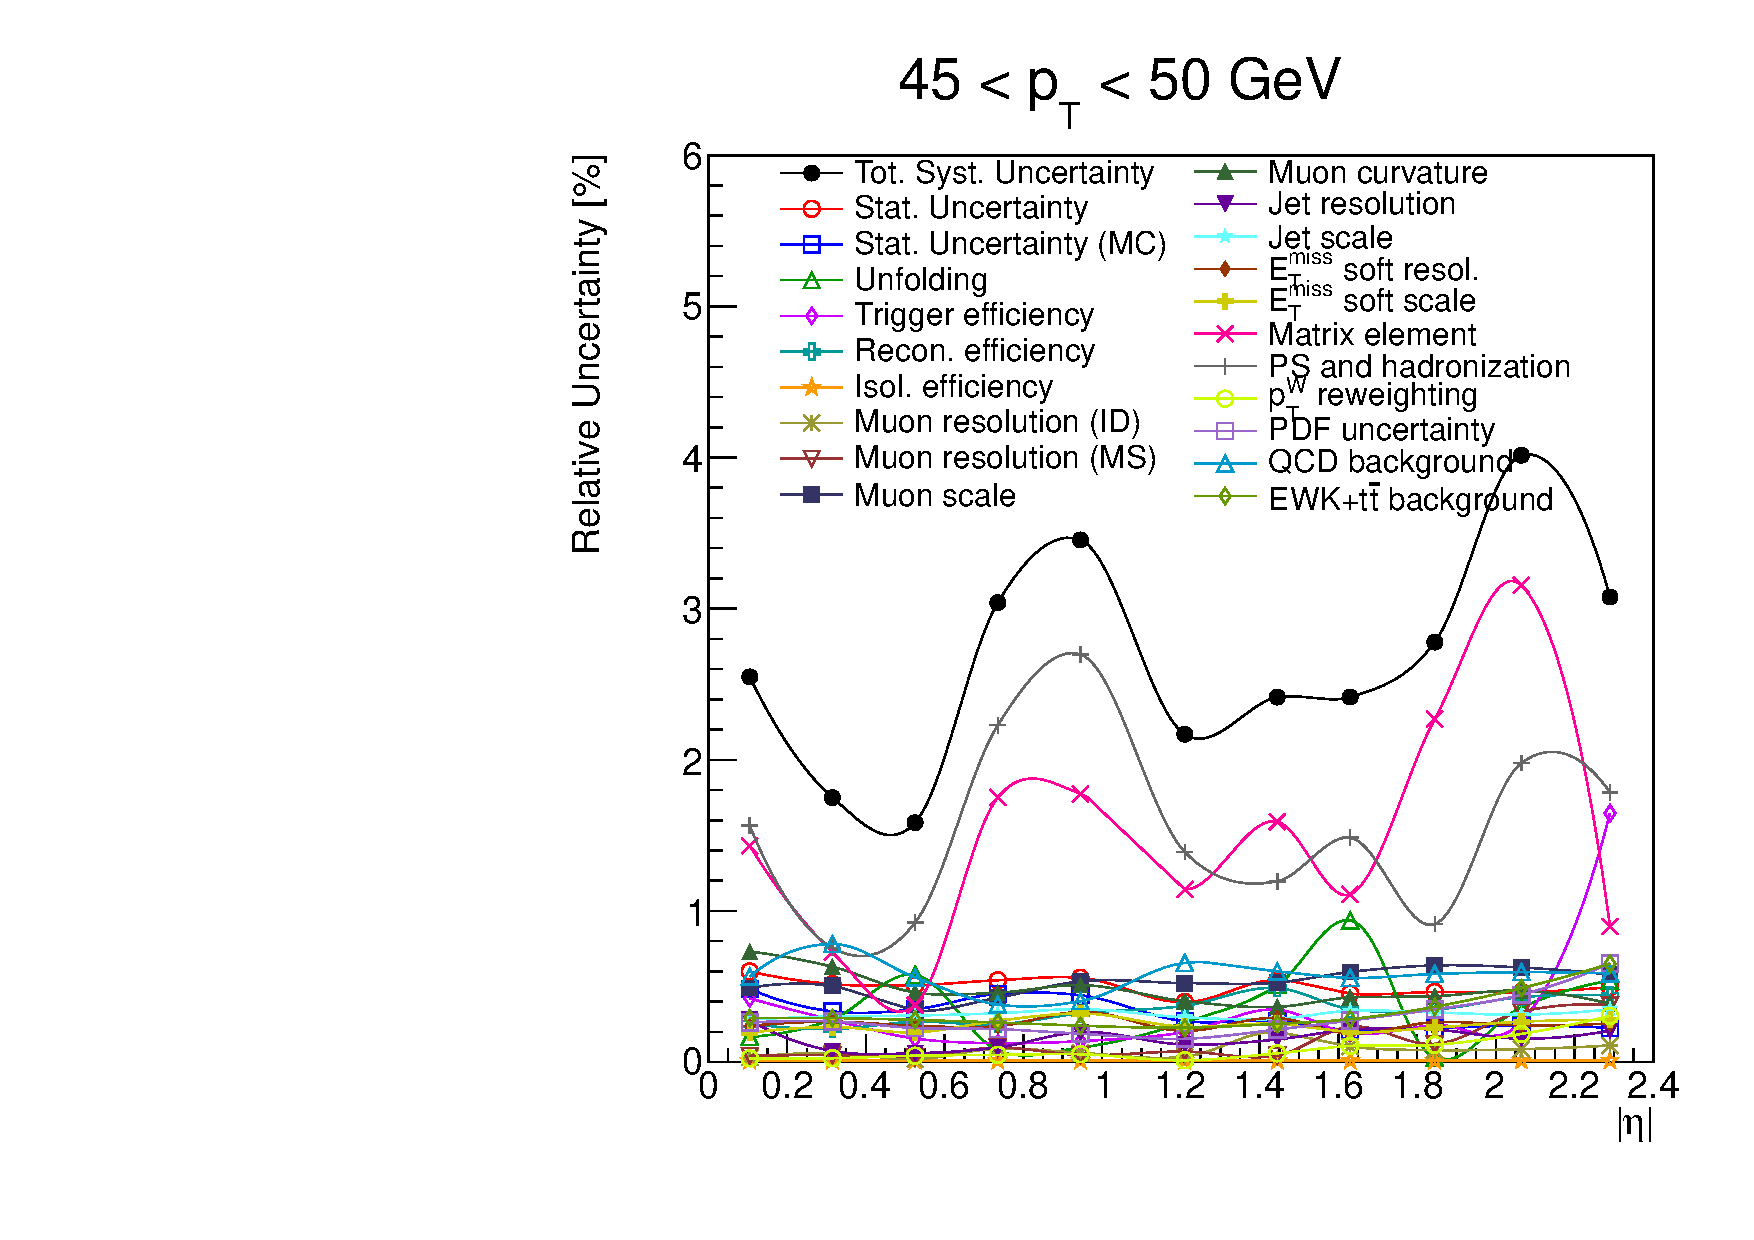
\includegraphics[width=0.3\textwidth]{dates/20121219/figures/xsec/POS/Wmn_Unc_2d_Slice_6.pdf}
   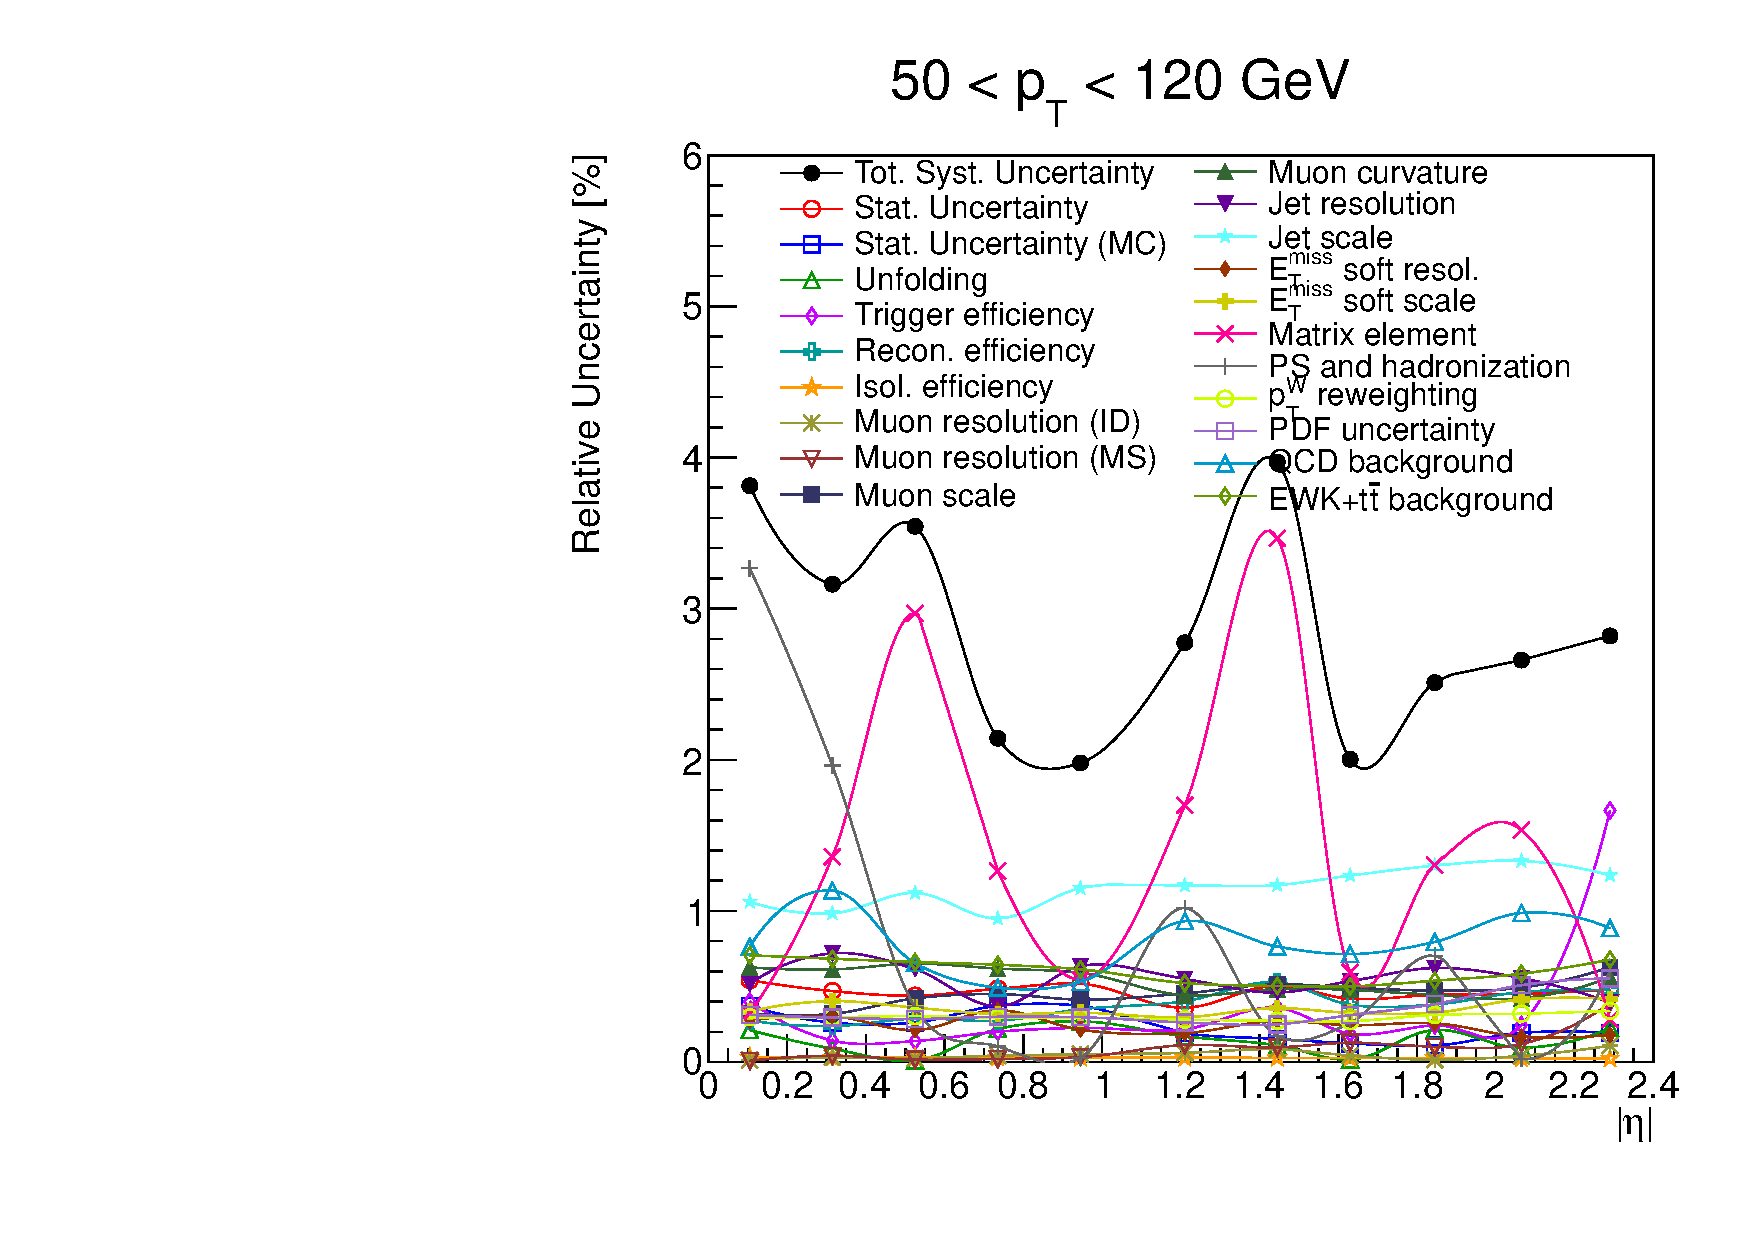
\includegraphics[width=0.3\textwidth]{dates/20121219/figures/xsec/POS/Wmn_Unc_2d_Slice_7.pdf}
 \end{center}
\end{frame}



\section{ Double-differential NEG }

\begin{frame}{Unfolded cros-sections: $\Wminus \rightarrow \mu^- \nu$}
 \begin{center}
   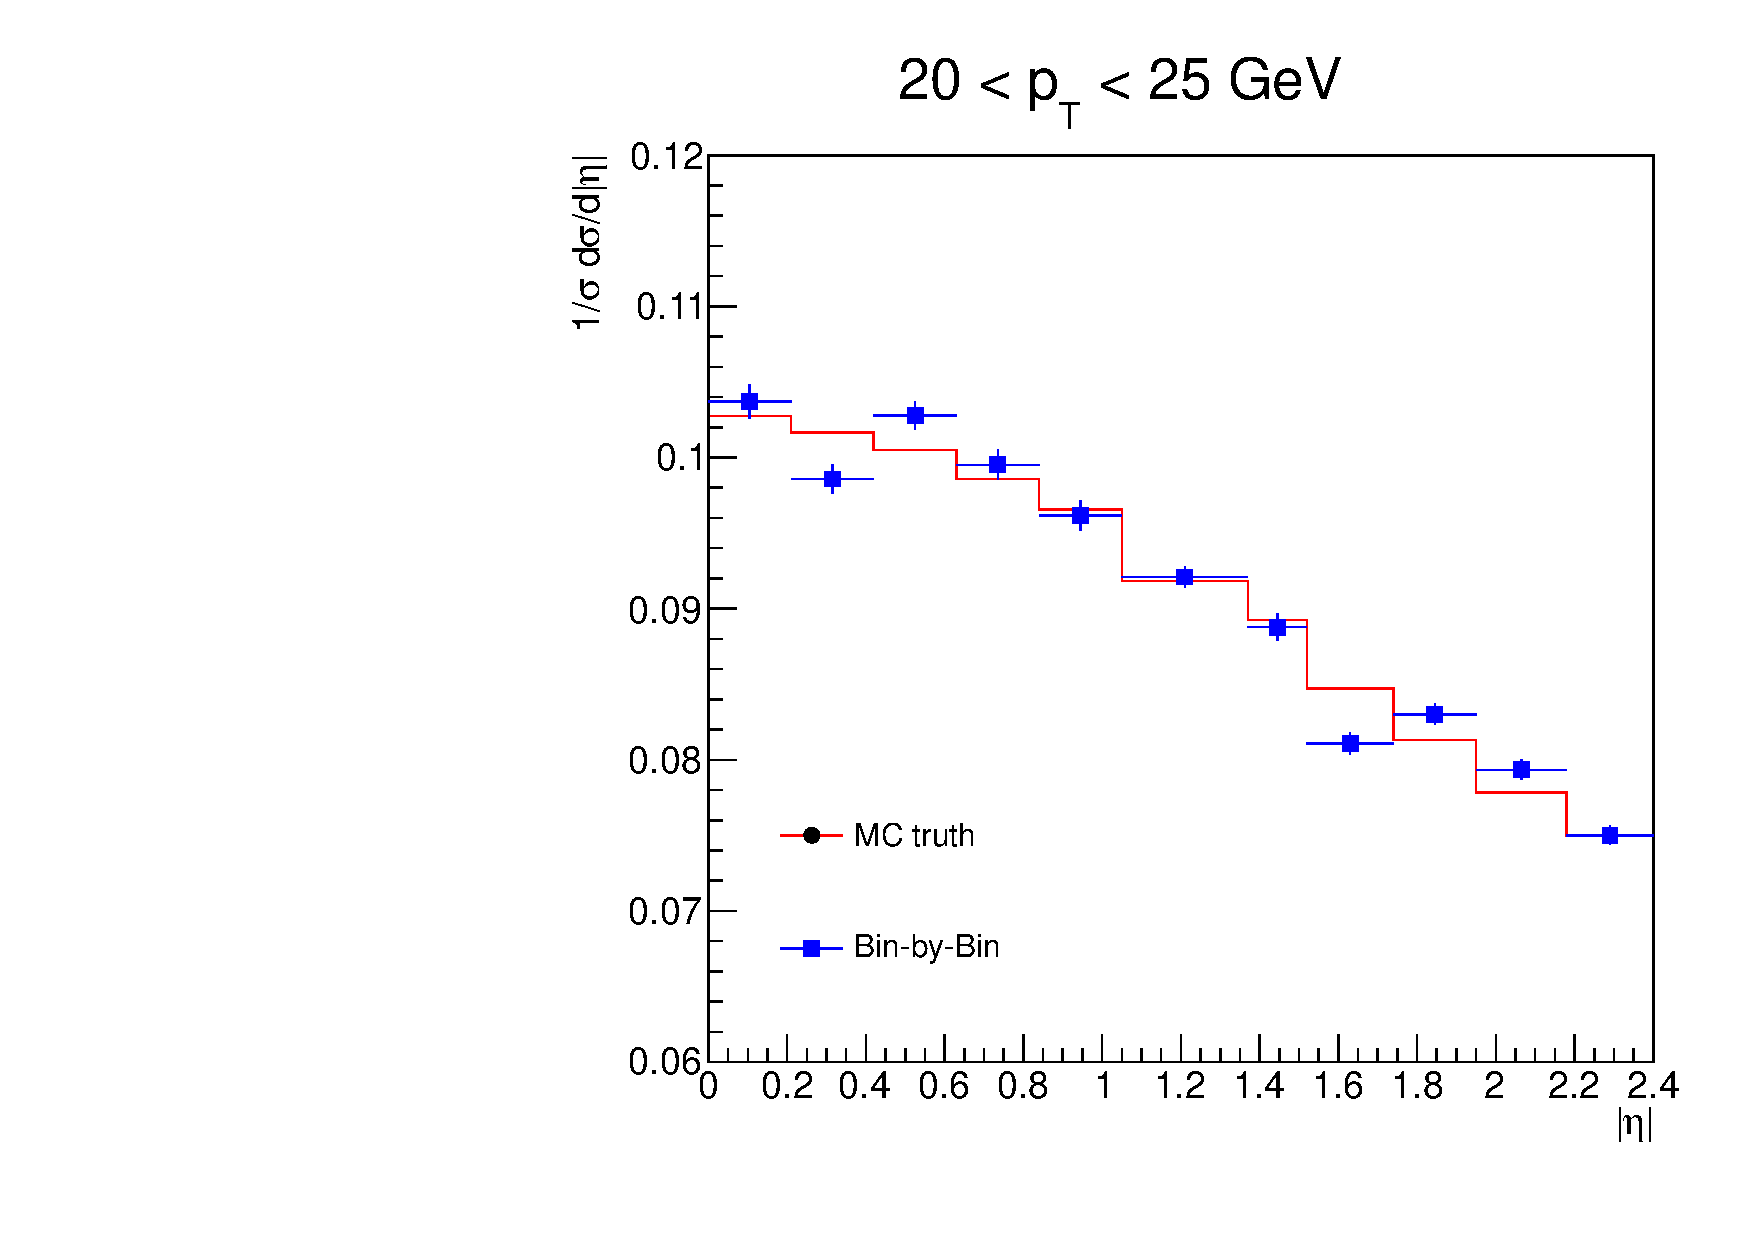
\includegraphics[width=0.6\textwidth]{dates/20121219/figures/xsec/NEG/Wmn_Unf_2d_Slice_1.pdf}
 \end{center}
\end{frame}

\begin{frame}{Unfolded cross-sections: $\Wminus \rightarrow \mu^- \nu$}
 \begin{center}
   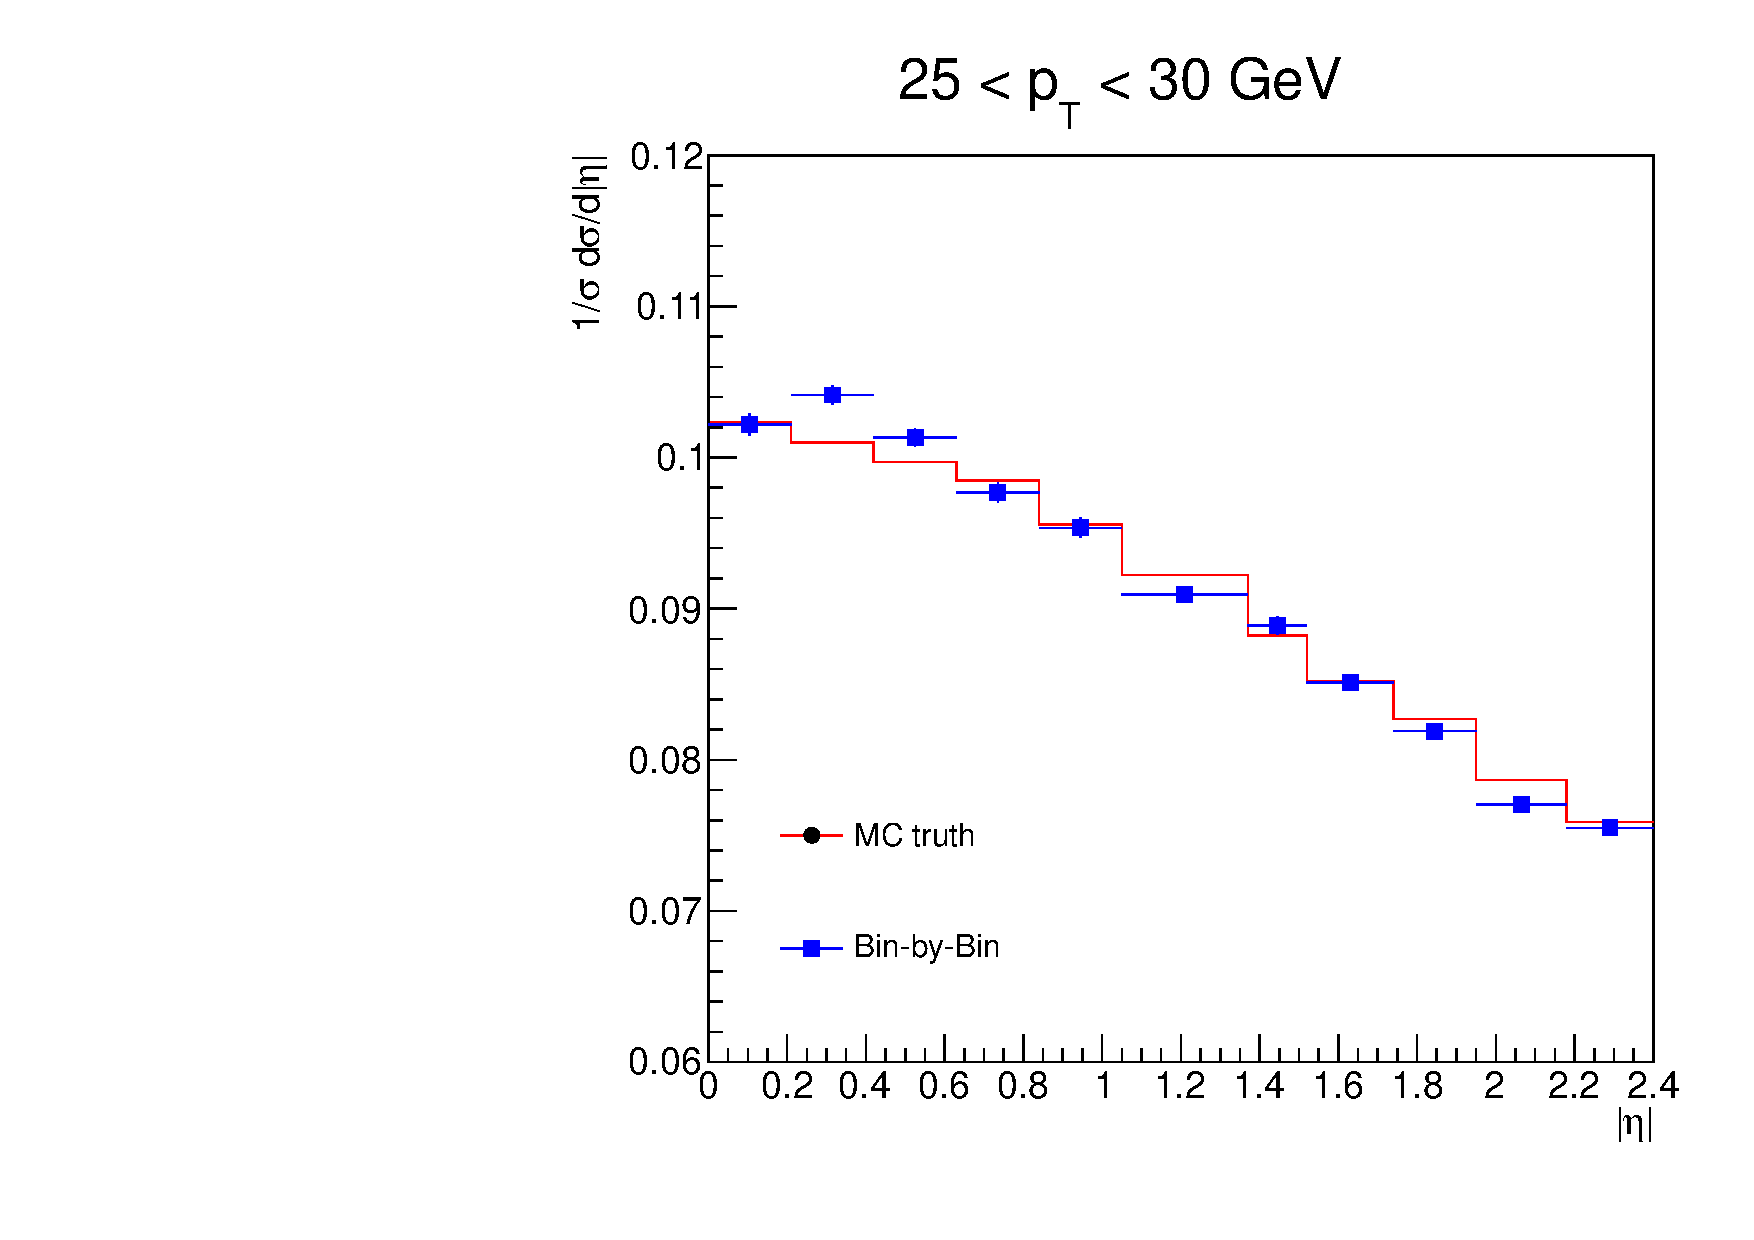
\includegraphics[width=0.3\textwidth]{dates/20121219/figures/xsec/NEG/Wmn_Unf_2d_Slice_2.pdf}
   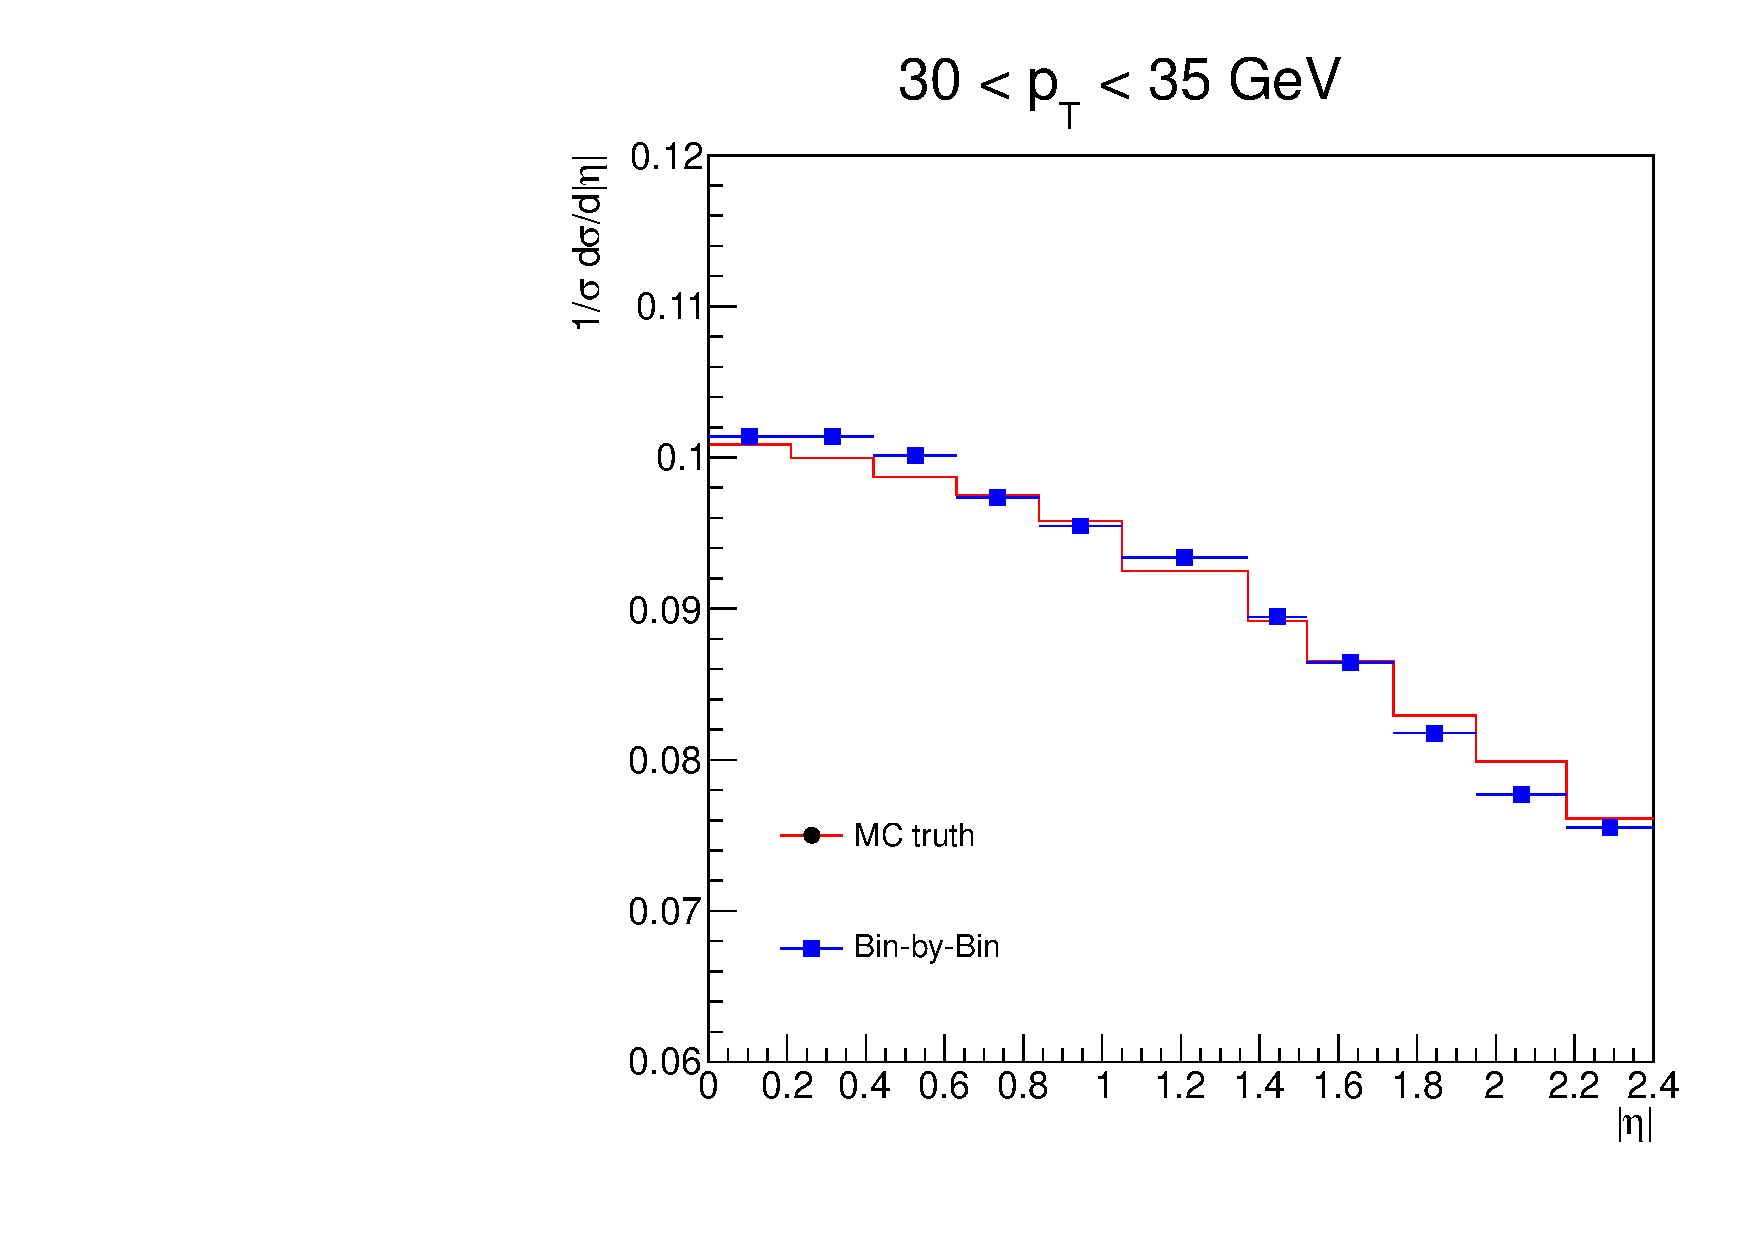
\includegraphics[width=0.3\textwidth]{dates/20121219/figures/xsec/NEG/Wmn_Unf_2d_Slice_3.pdf}
   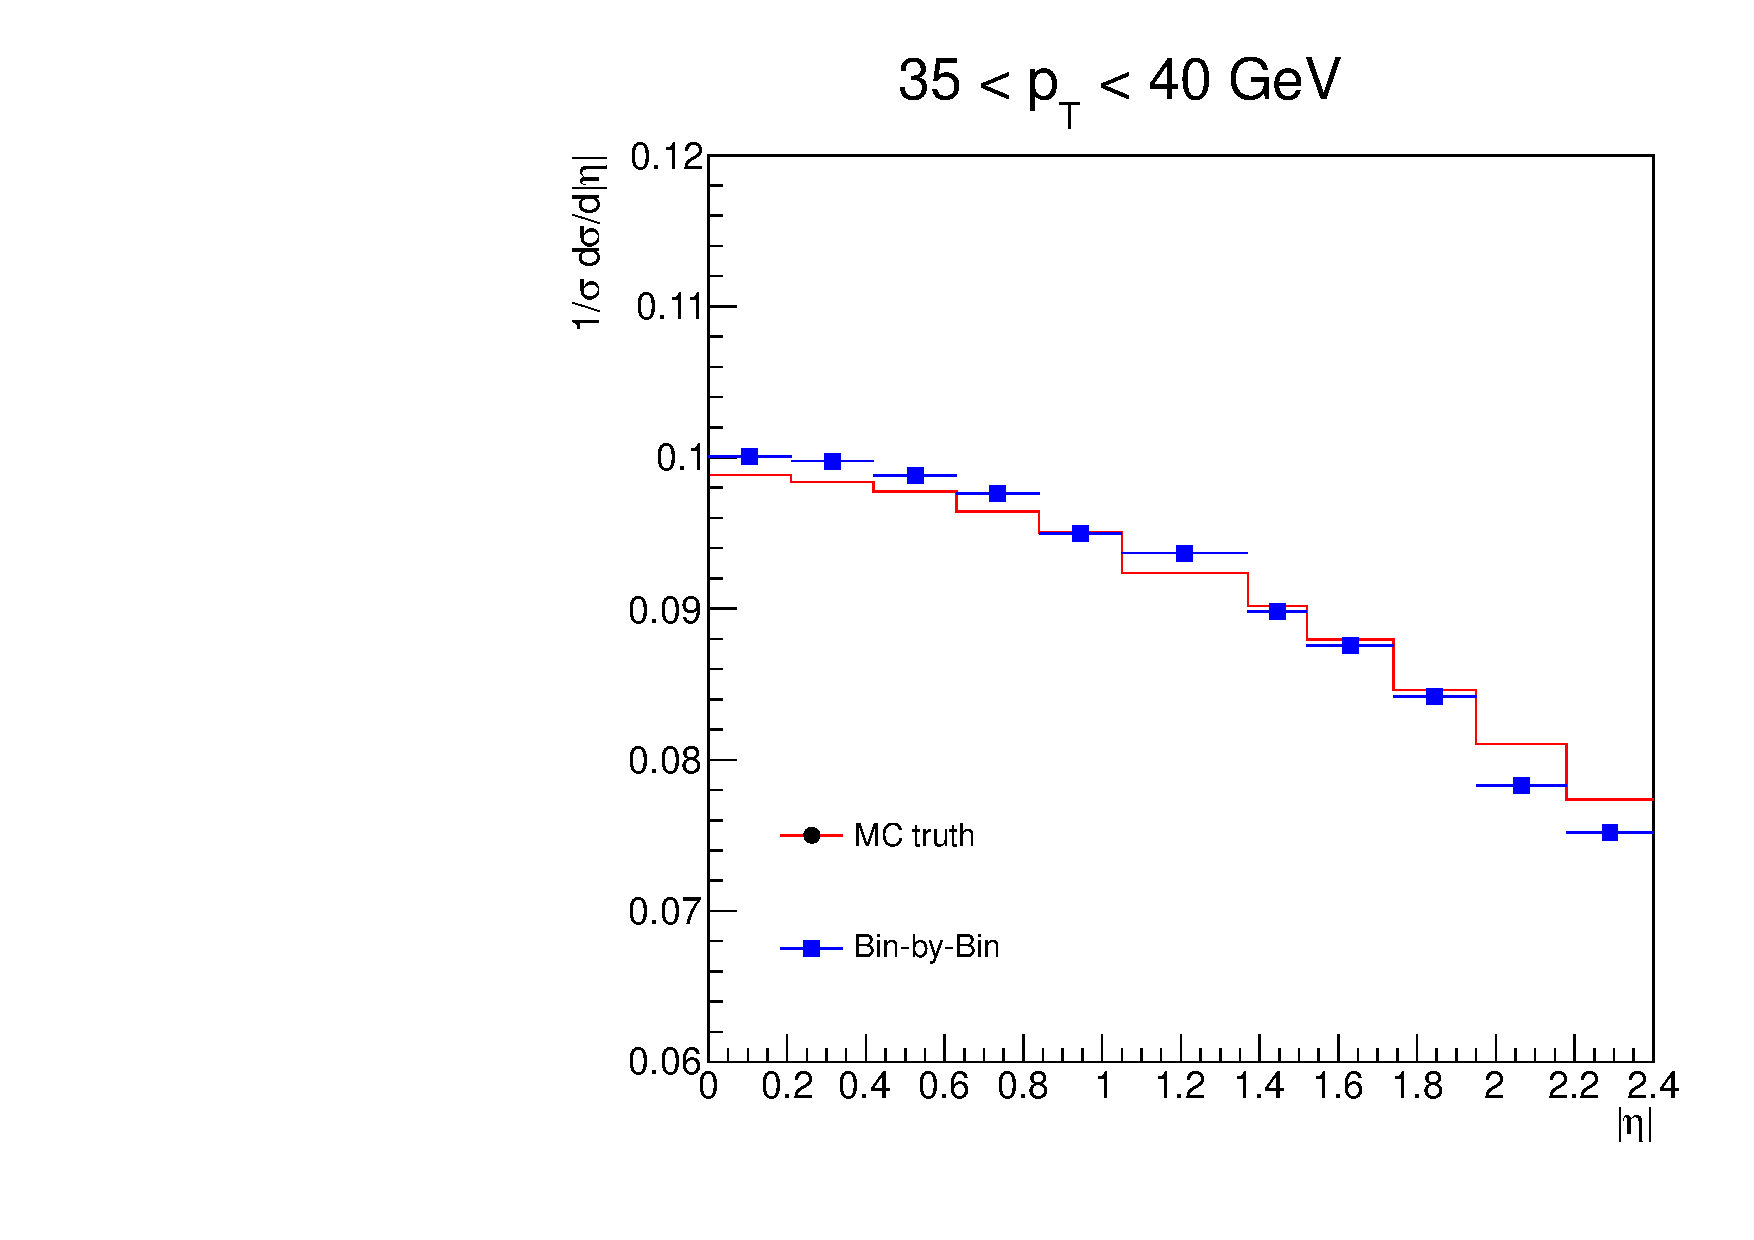
\includegraphics[width=0.3\textwidth]{dates/20121219/figures/xsec/NEG/Wmn_Unf_2d_Slice_4.pdf}
 \end{center}
 \begin{center}
   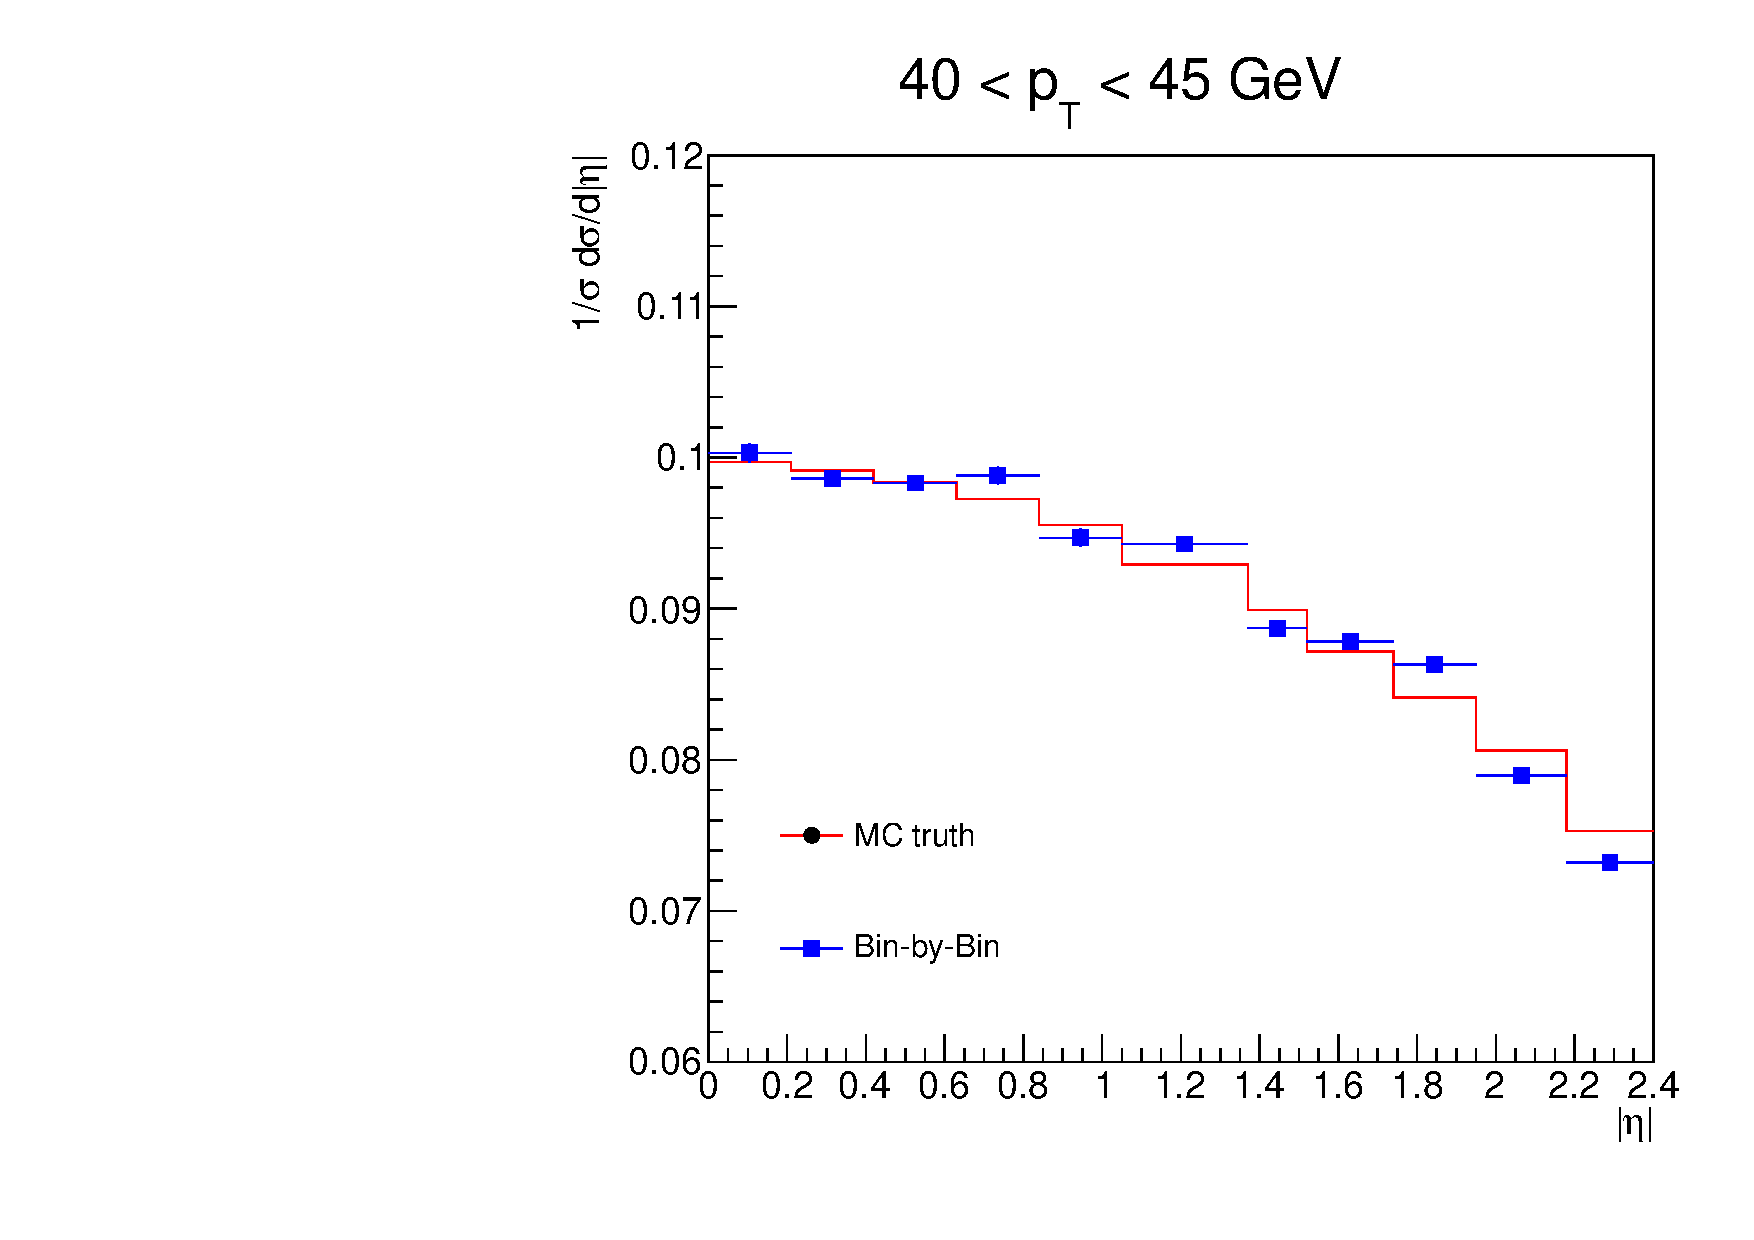
\includegraphics[width=0.3\textwidth]{dates/20121219/figures/xsec/NEG/Wmn_Unf_2d_Slice_5.pdf}
   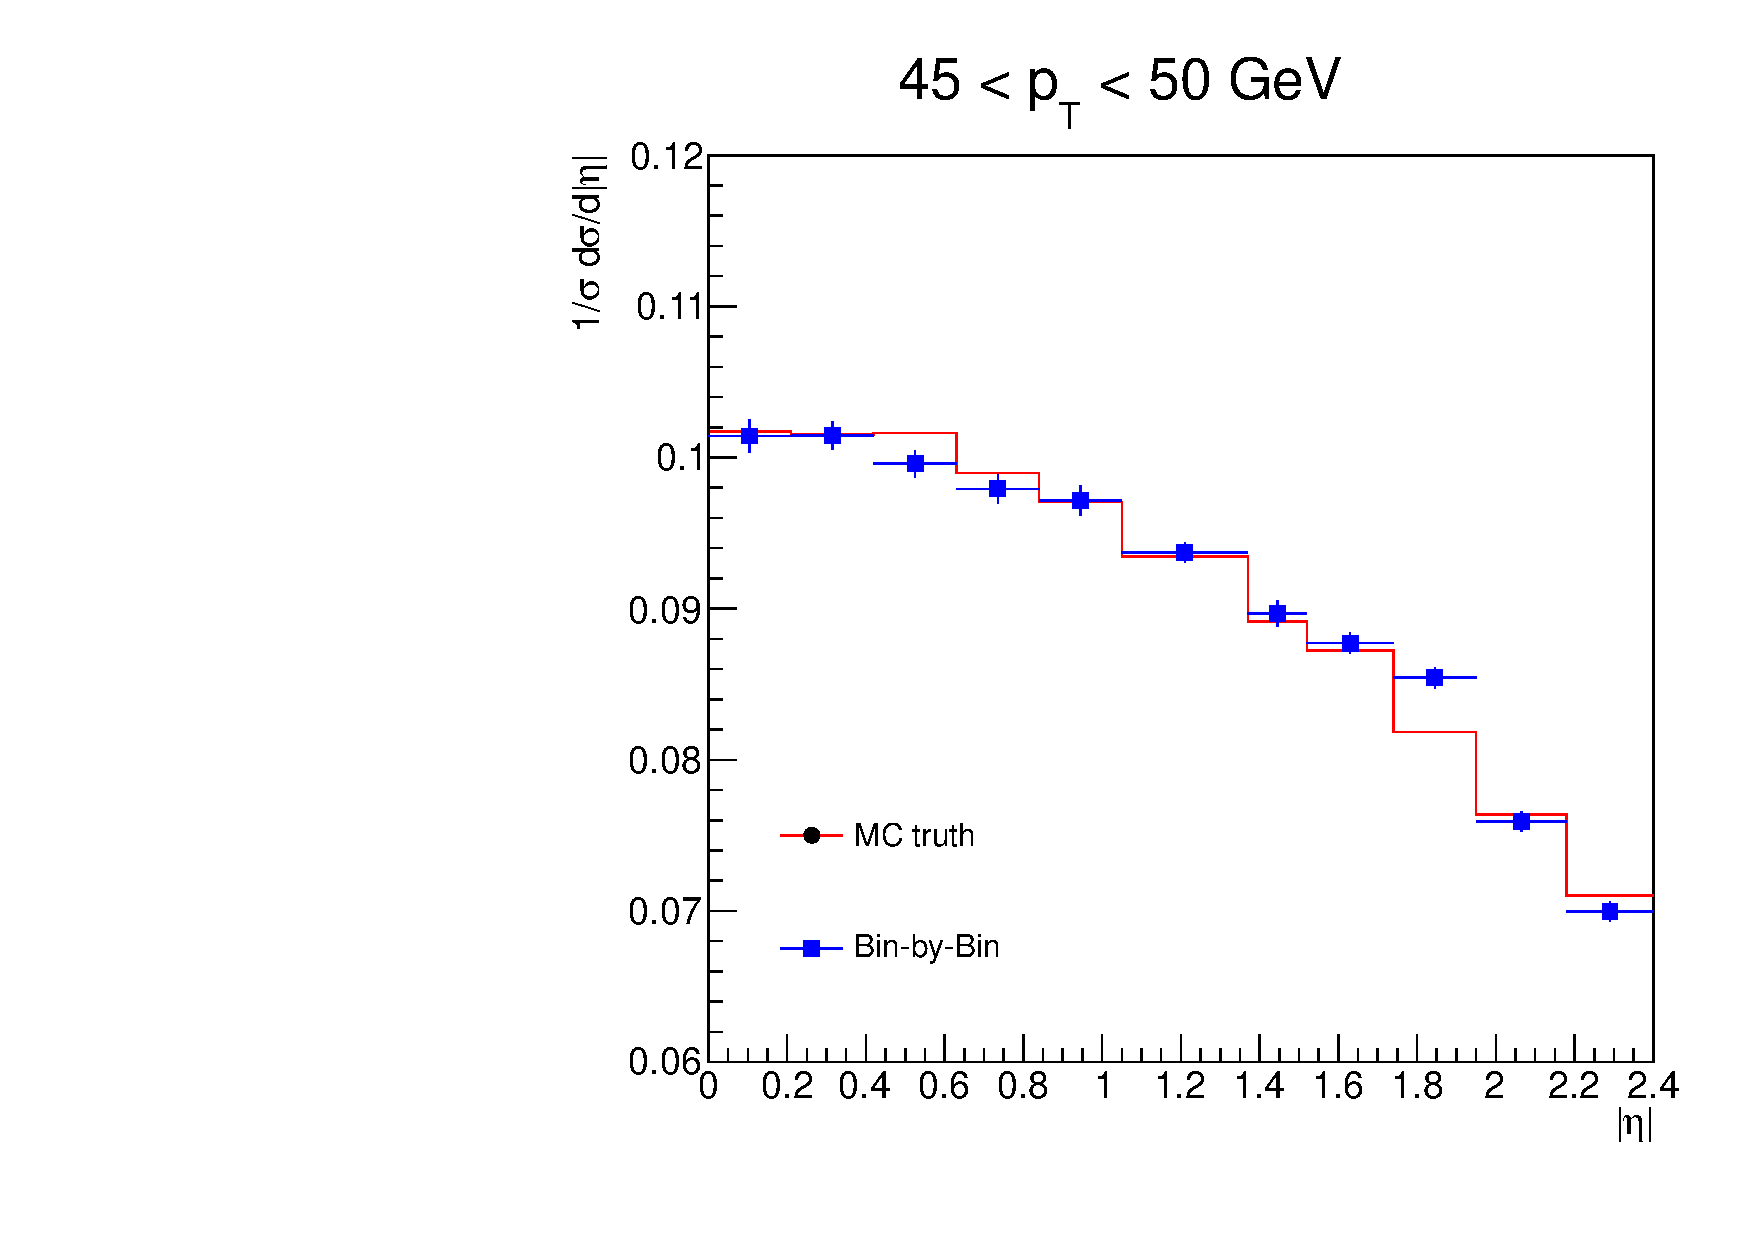
\includegraphics[width=0.3\textwidth]{dates/20121219/figures/xsec/NEG/Wmn_Unf_2d_Slice_6.pdf}
   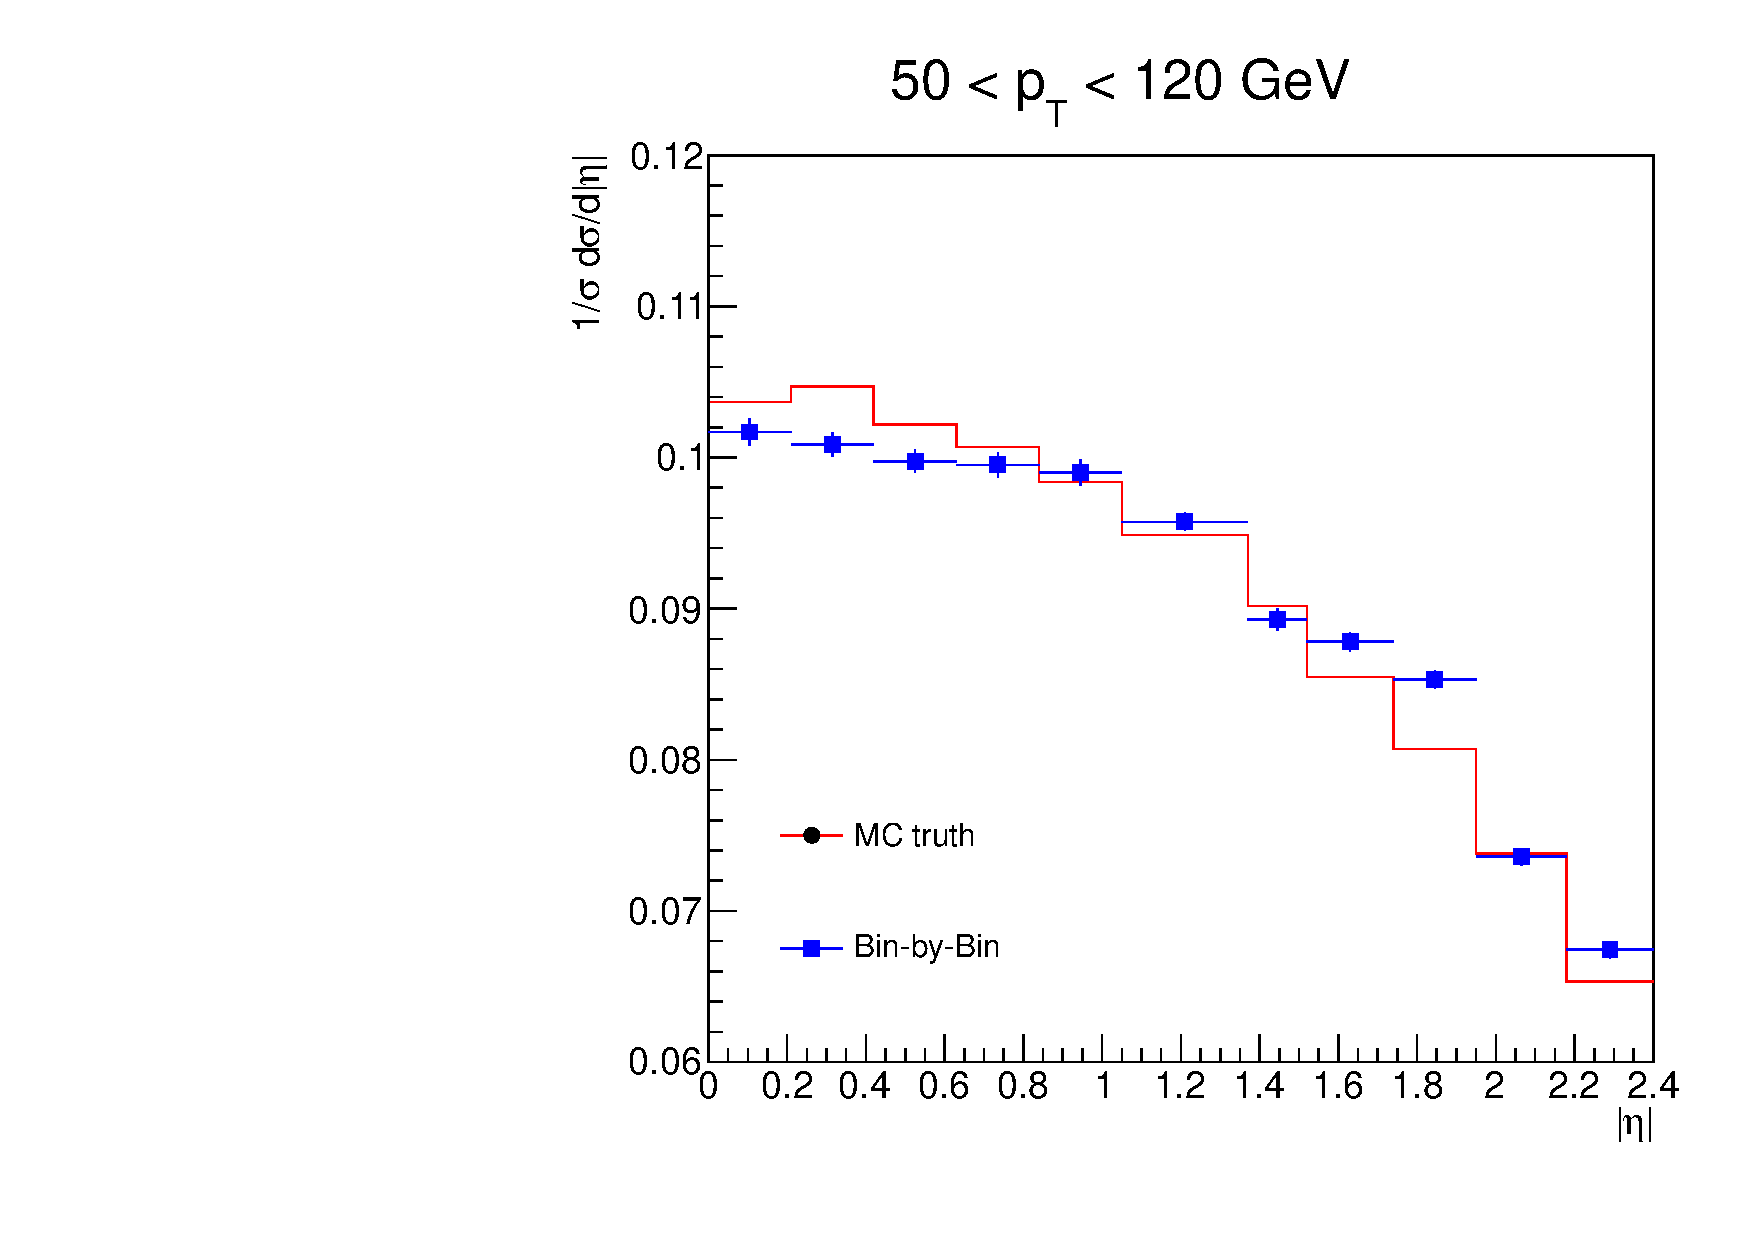
\includegraphics[width=0.3\textwidth]{dates/20121219/figures/xsec/NEG/Wmn_Unf_2d_Slice_7.pdf}
 \end{center}
\end{frame}



\begin{frame}{Systematic Uncertainties: $\Wminus \rightarrow \mu^- \nu$}
 \begin{center}
   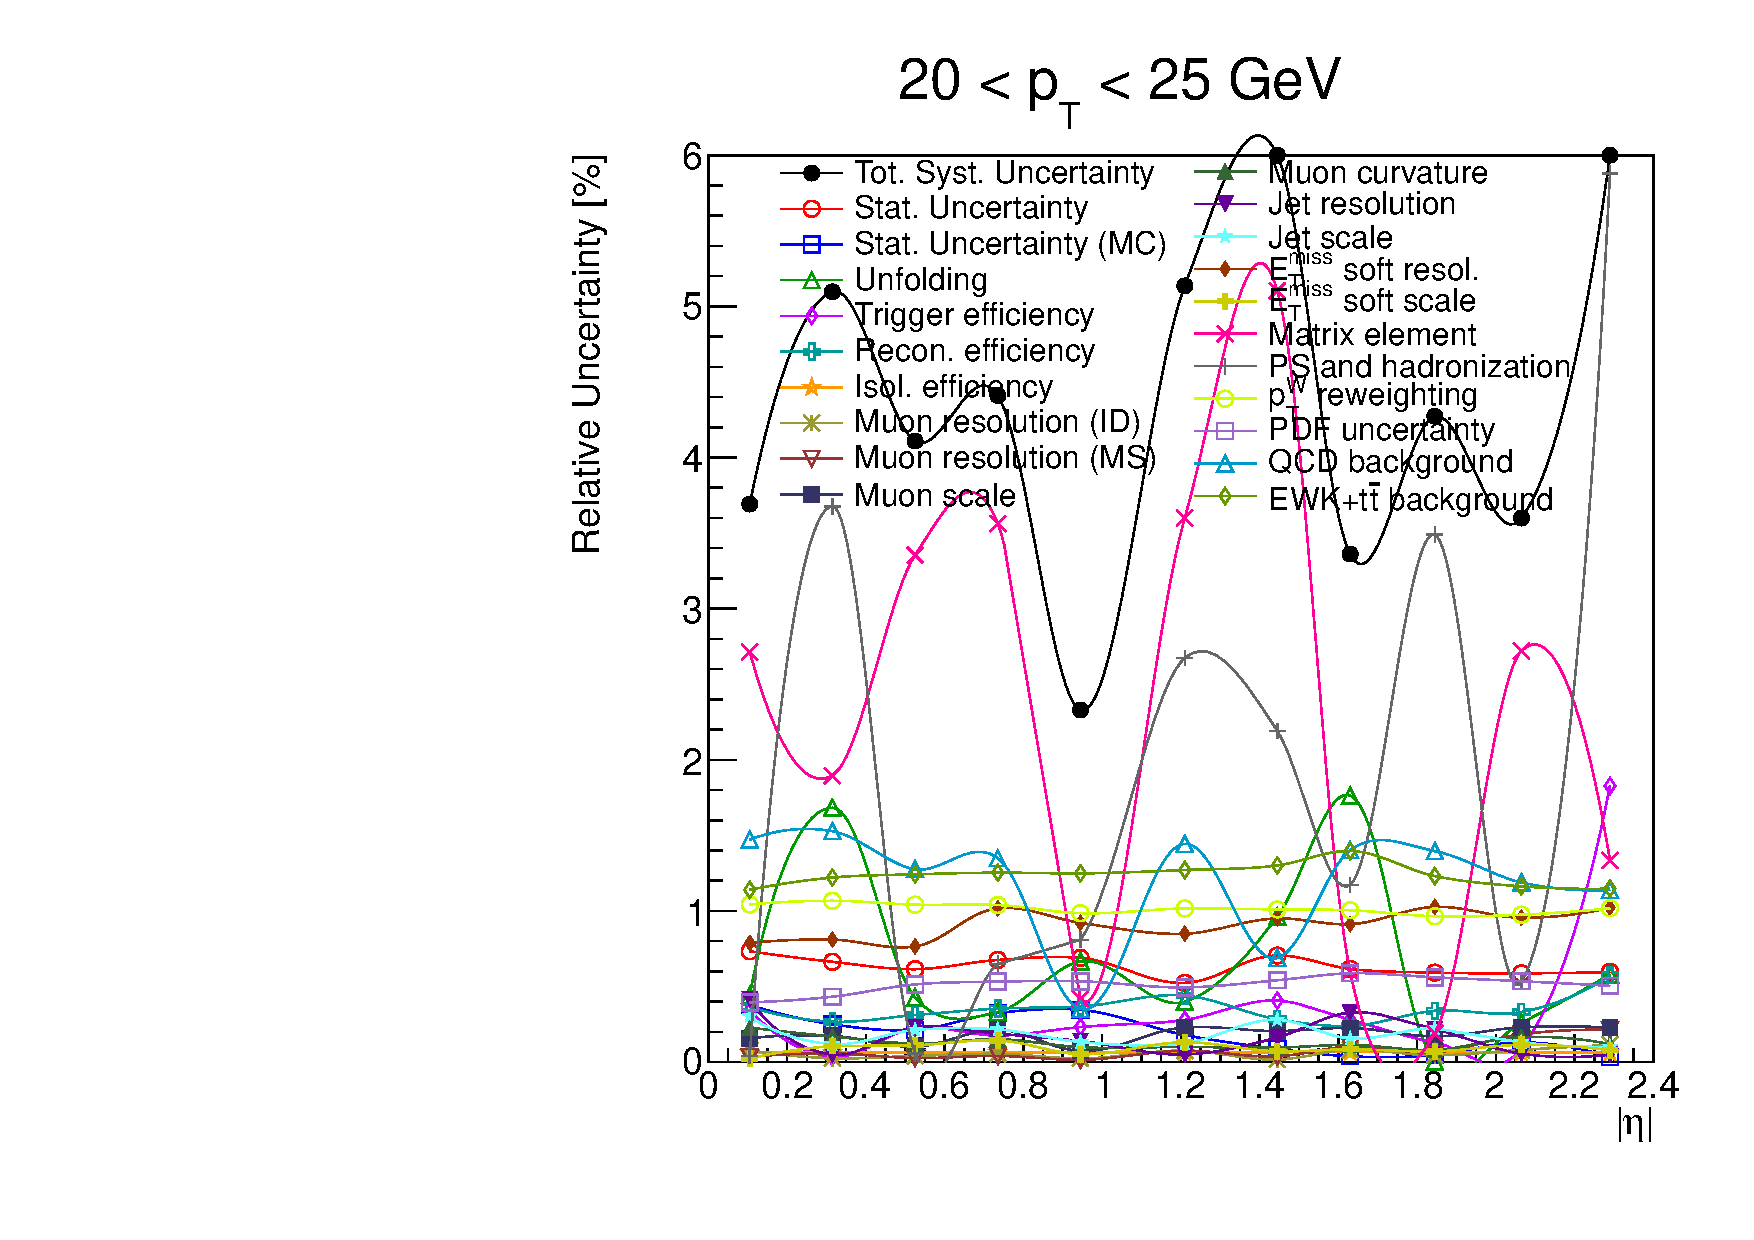
\includegraphics[width=0.6\textwidth]{dates/20121219/figures/xsec/NEG/Wmn_Unc_2d_Slice_1.pdf}
 \end{center}
\end{frame}

\begin{frame}{Systematic Uncertainties: $\Wminus \rightarrow \mu^- \nu$}
 \begin{center}
   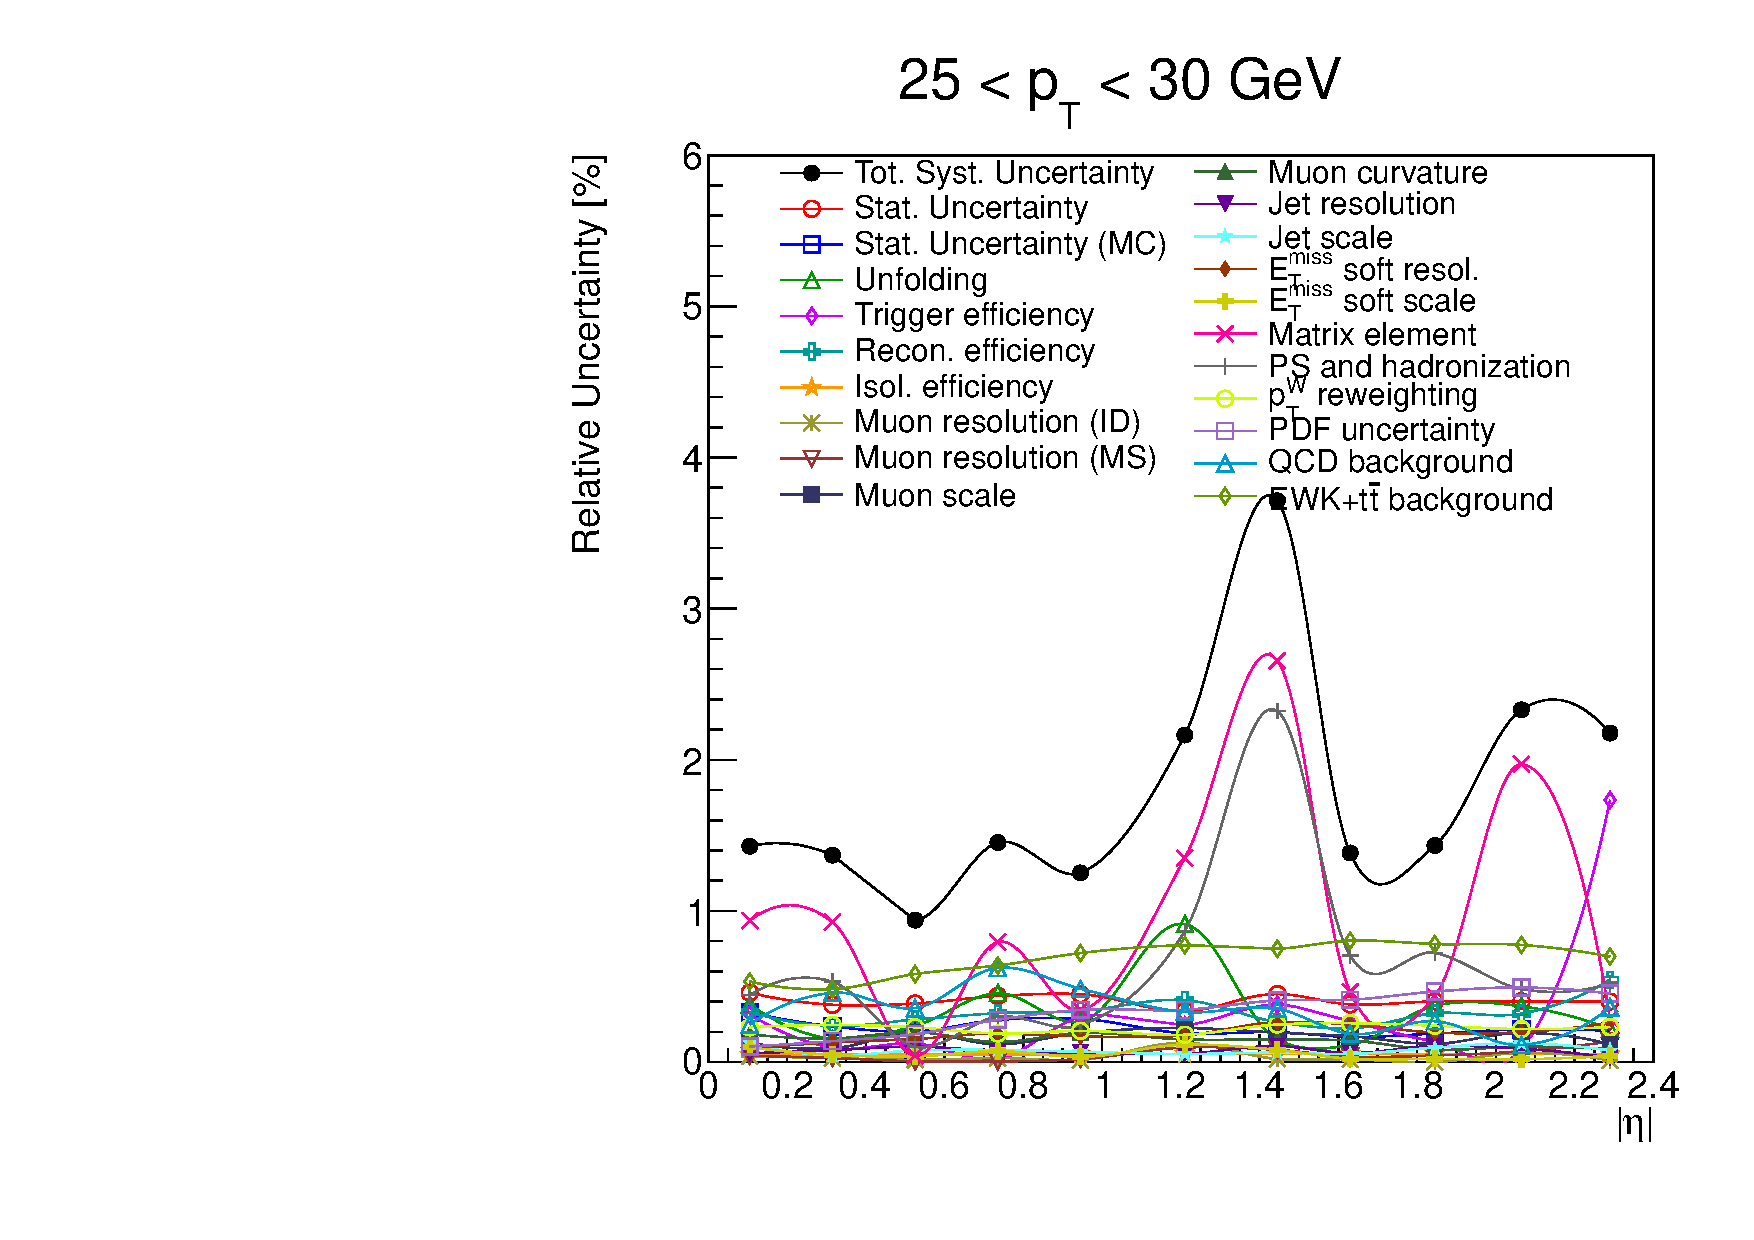
\includegraphics[width=0.3\textwidth]{dates/20121219/figures/xsec/NEG/Wmn_Unc_2d_Slice_2.pdf}
   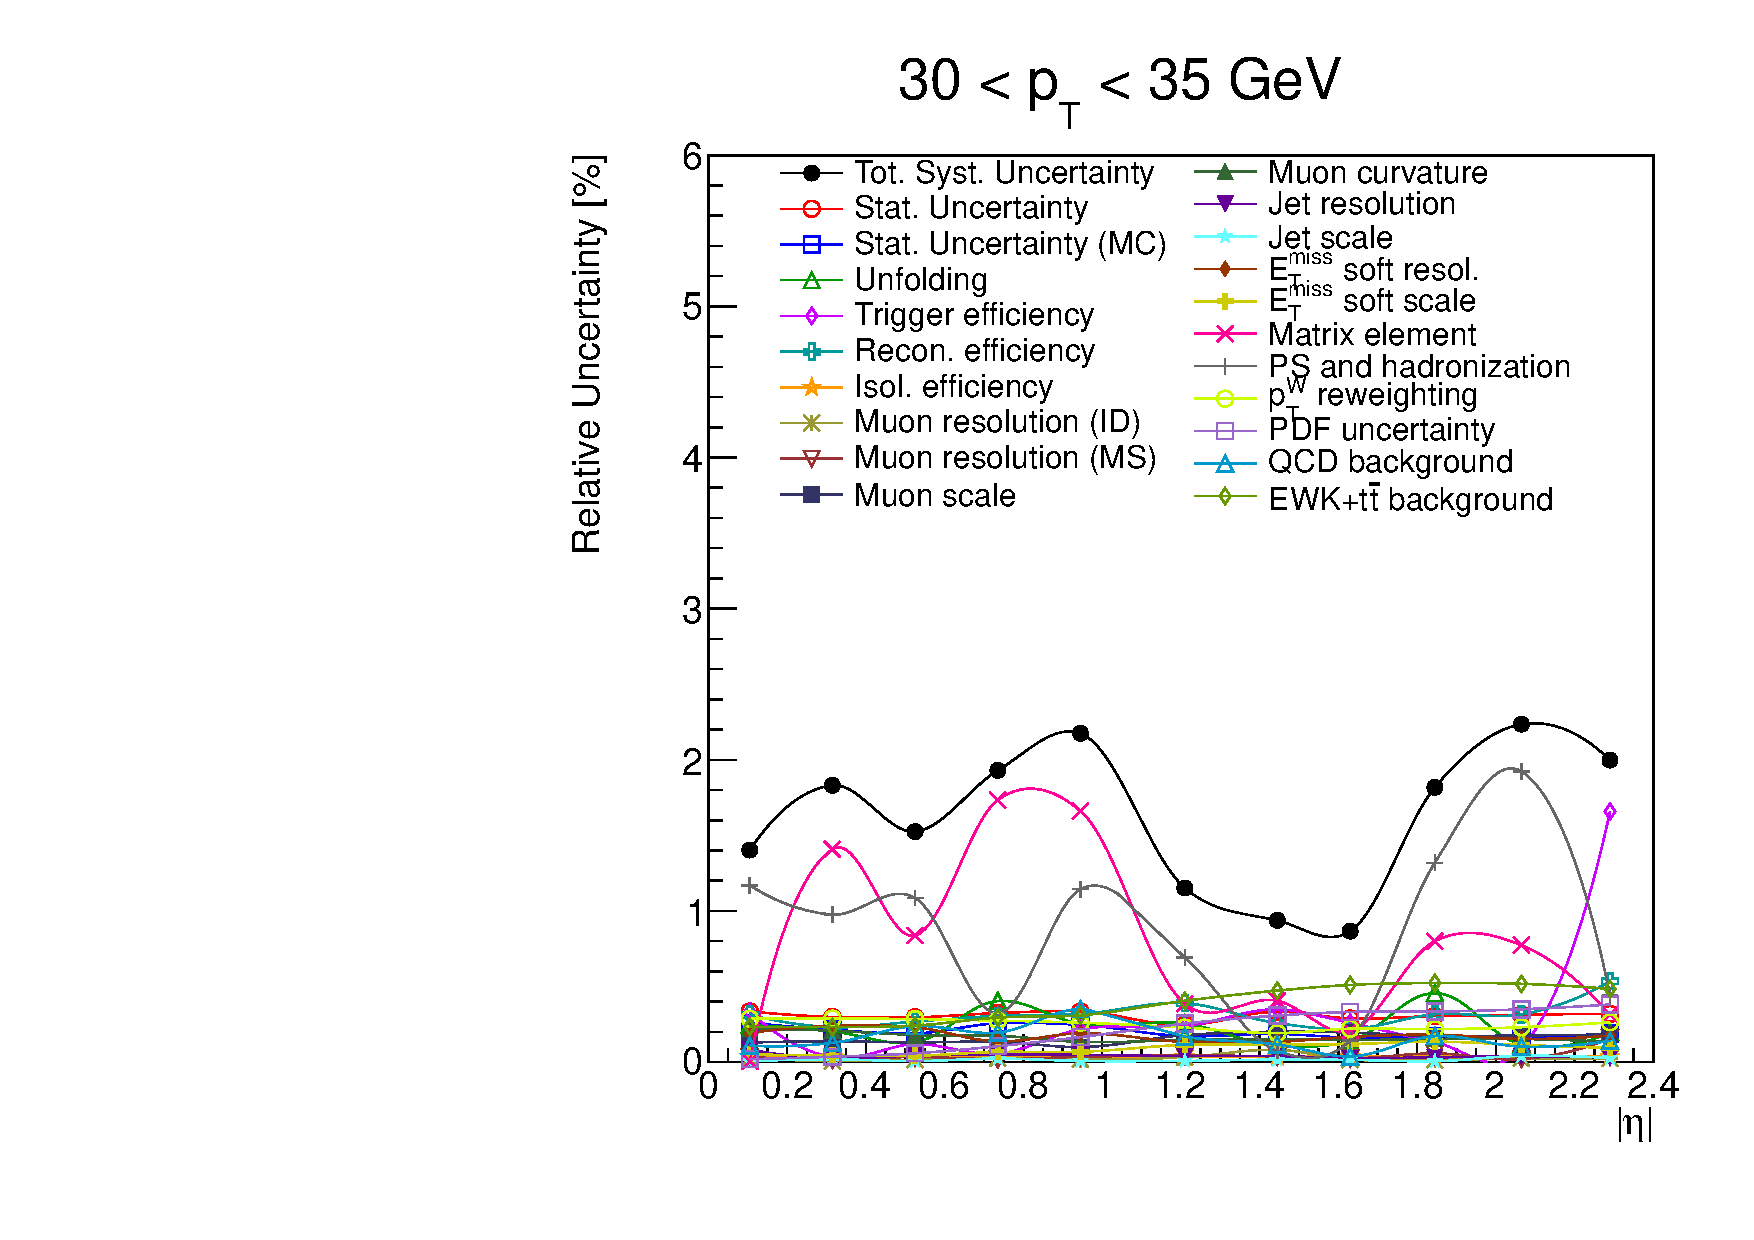
\includegraphics[width=0.3\textwidth]{dates/20121219/figures/xsec/NEG/Wmn_Unc_2d_Slice_3.pdf}
   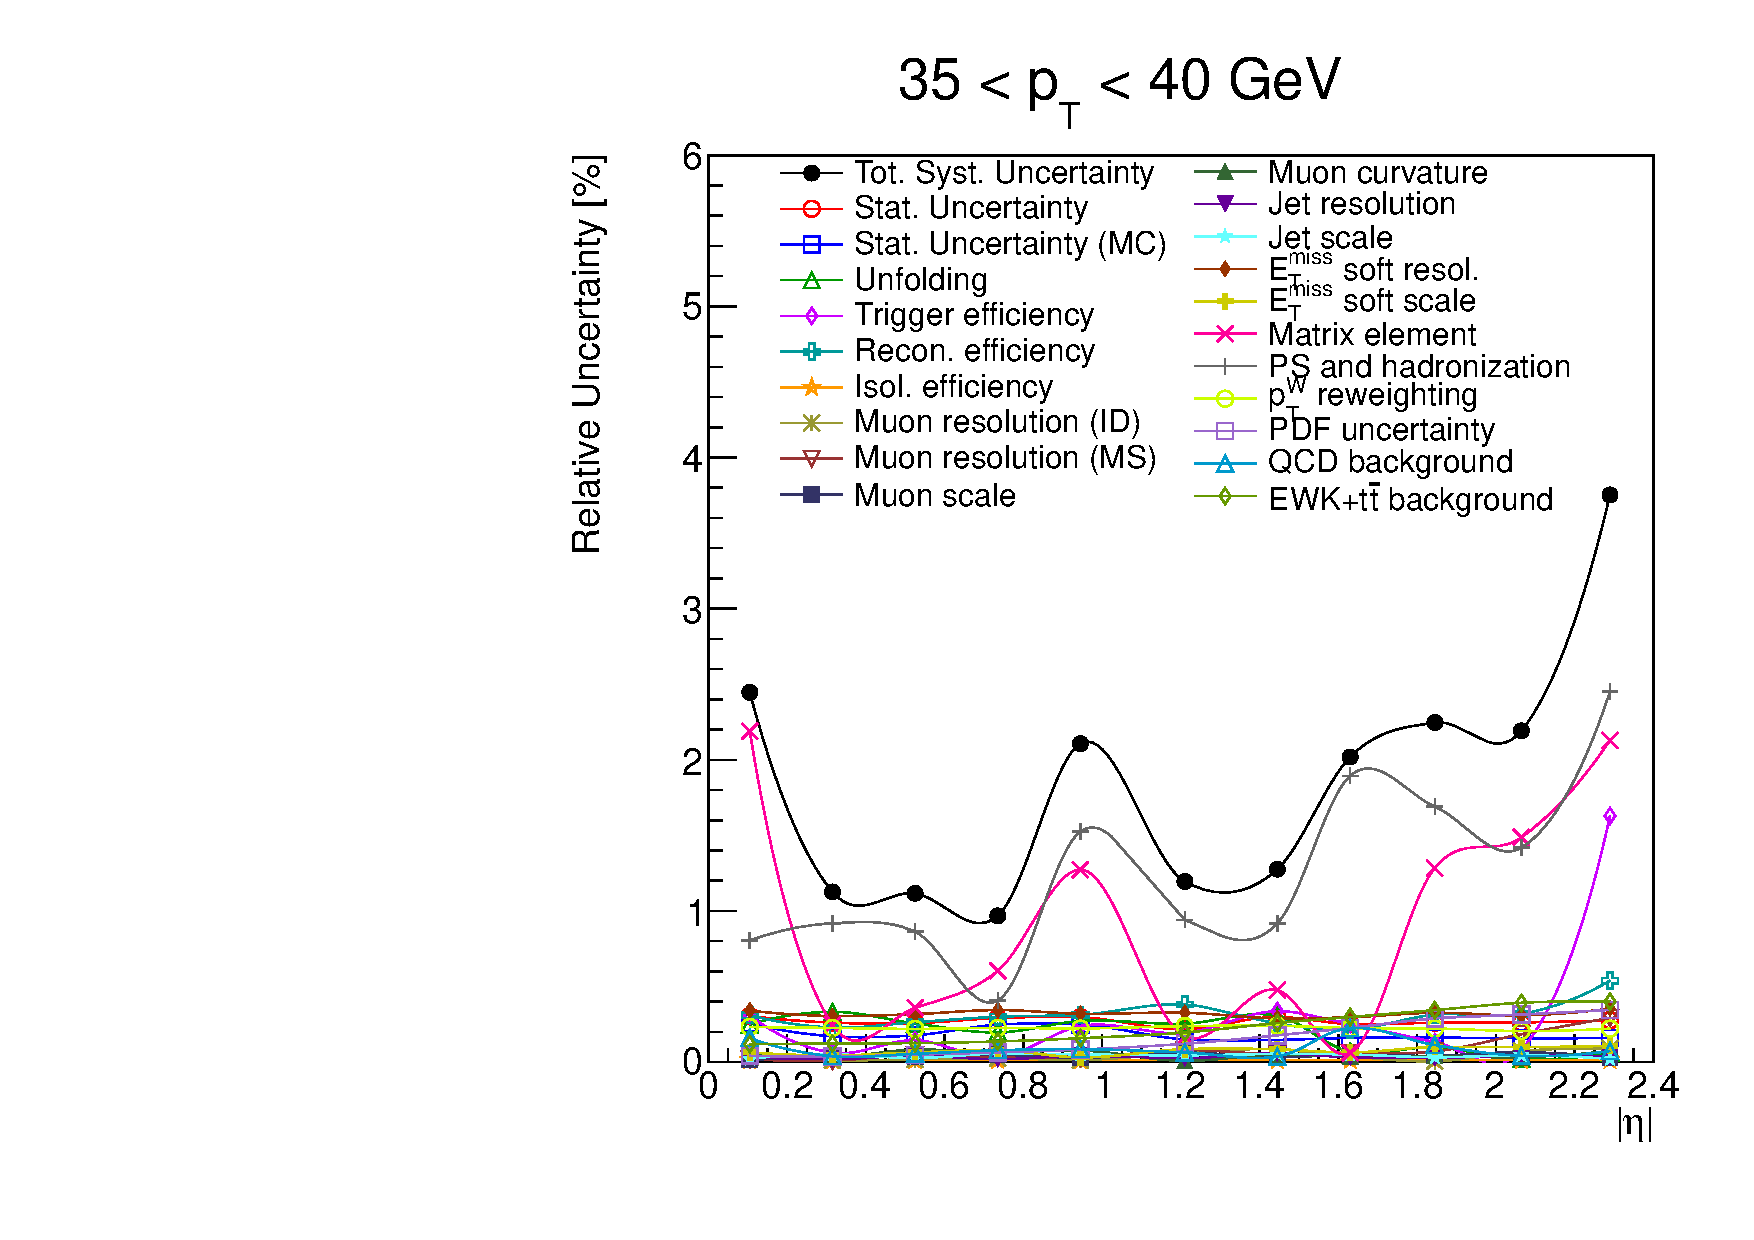
\includegraphics[width=0.3\textwidth]{dates/20121219/figures/xsec/NEG/Wmn_Unc_2d_Slice_4.pdf}
 \end{center}
 \begin{center}
   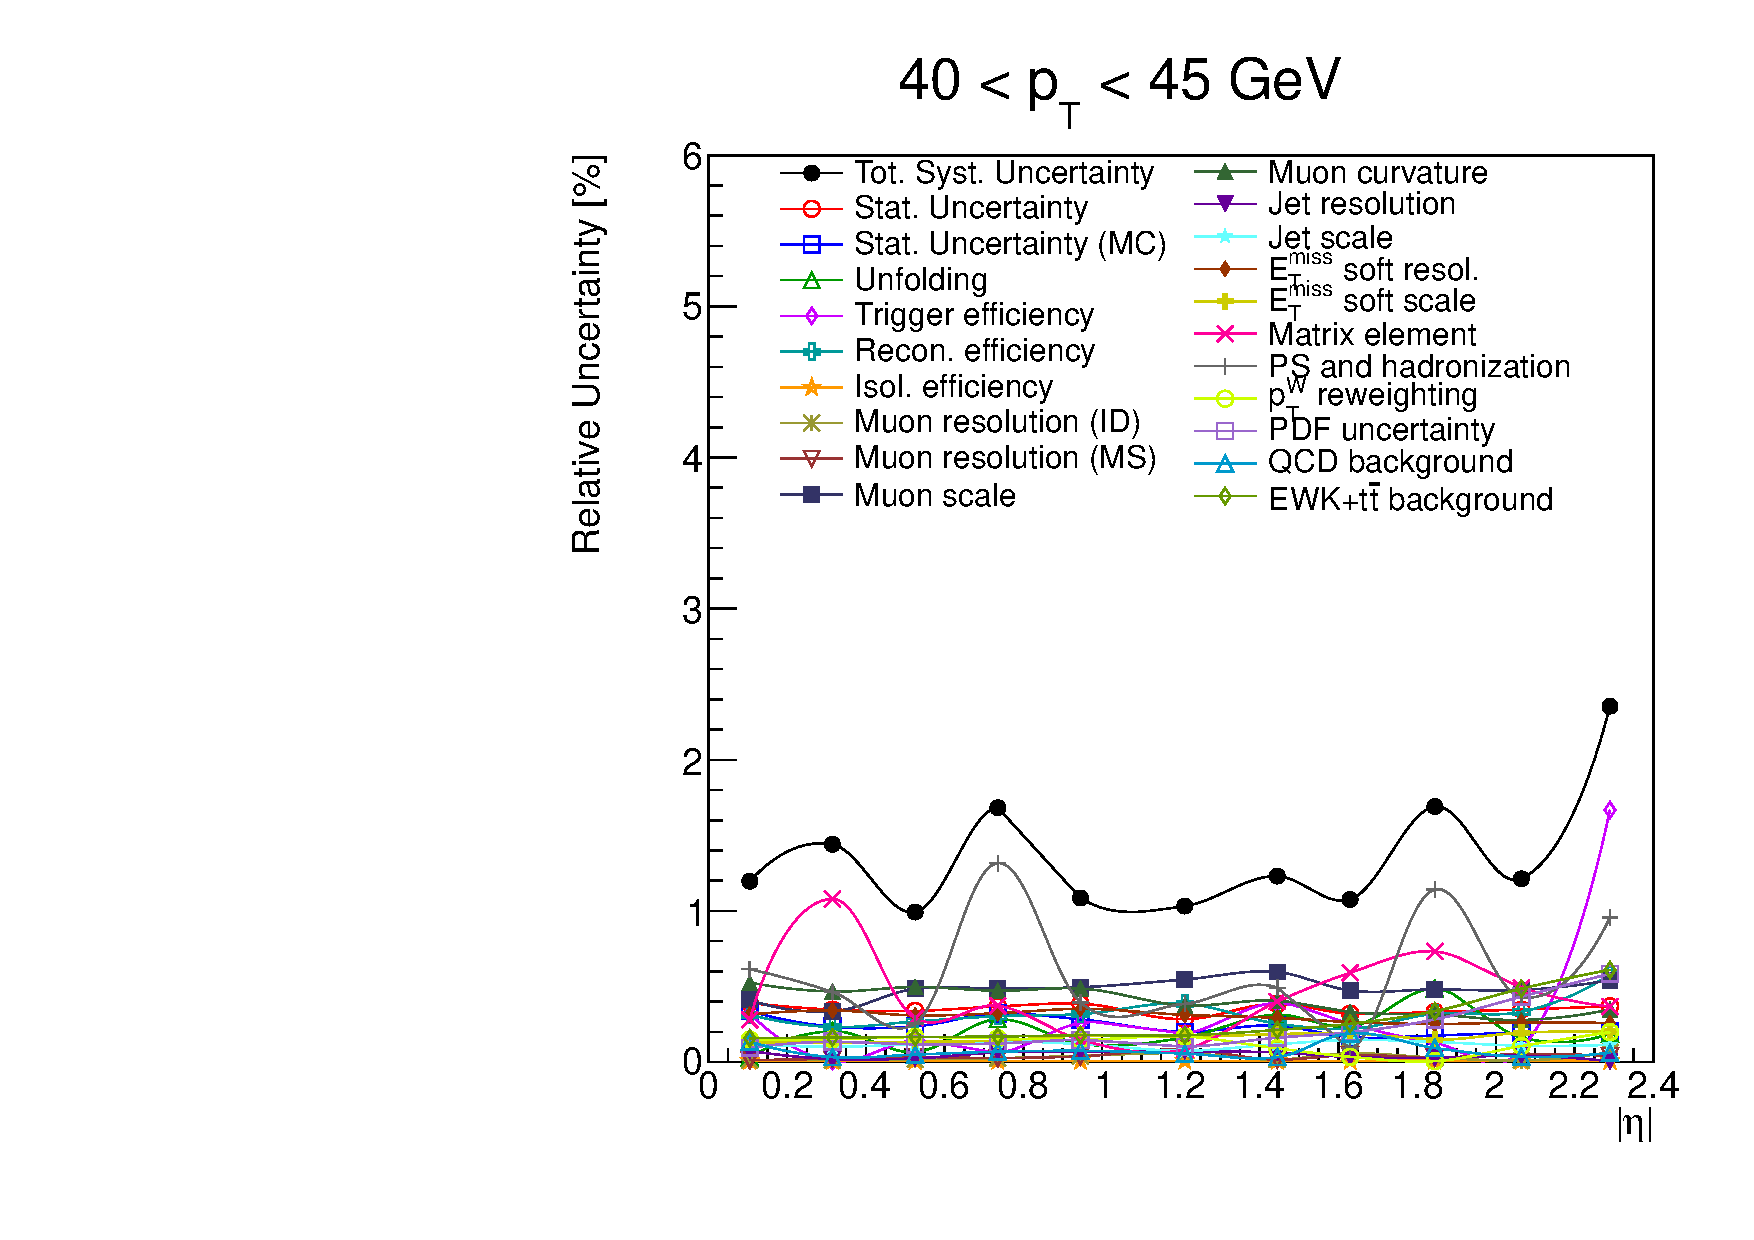
\includegraphics[width=0.3\textwidth]{dates/20121219/figures/xsec/NEG/Wmn_Unc_2d_Slice_5.pdf}
   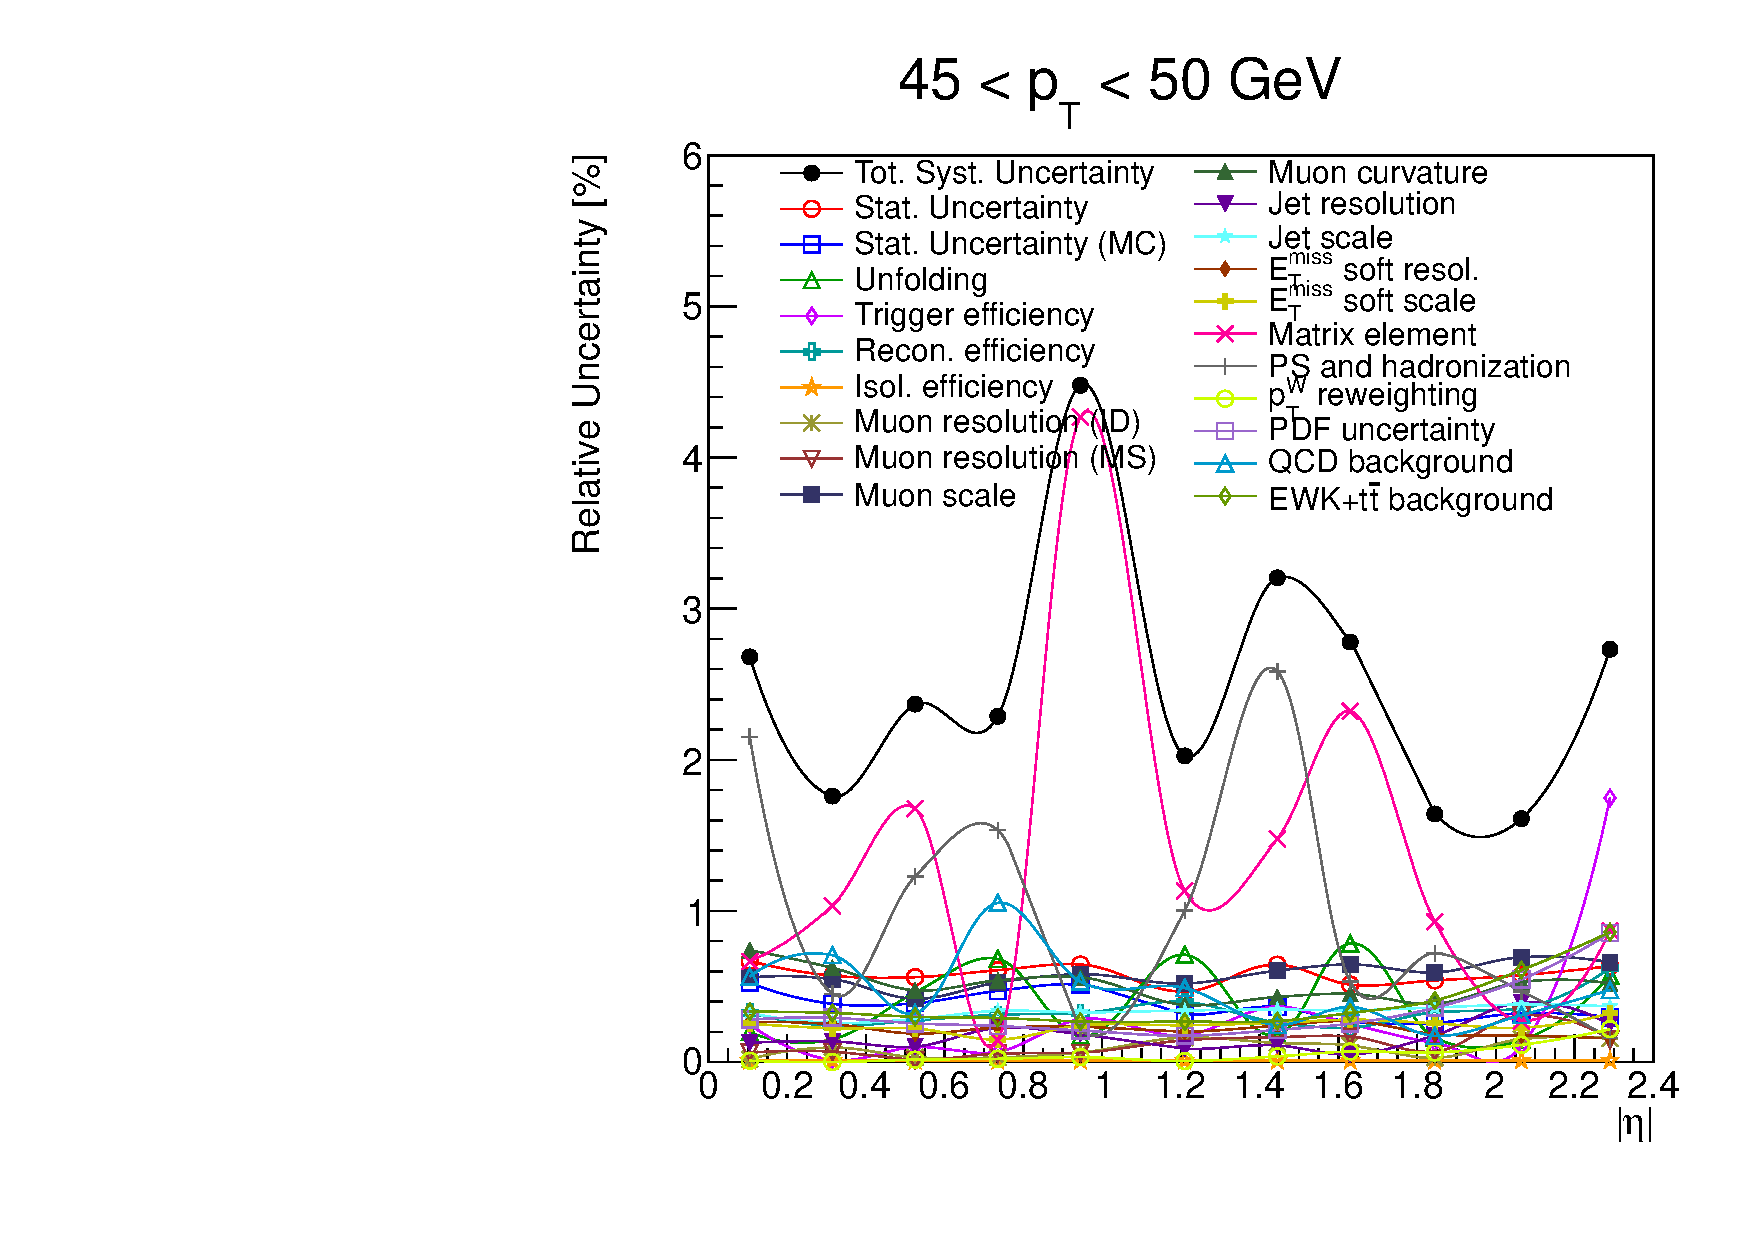
\includegraphics[width=0.3\textwidth]{dates/20121219/figures/xsec/NEG/Wmn_Unc_2d_Slice_6.pdf}
   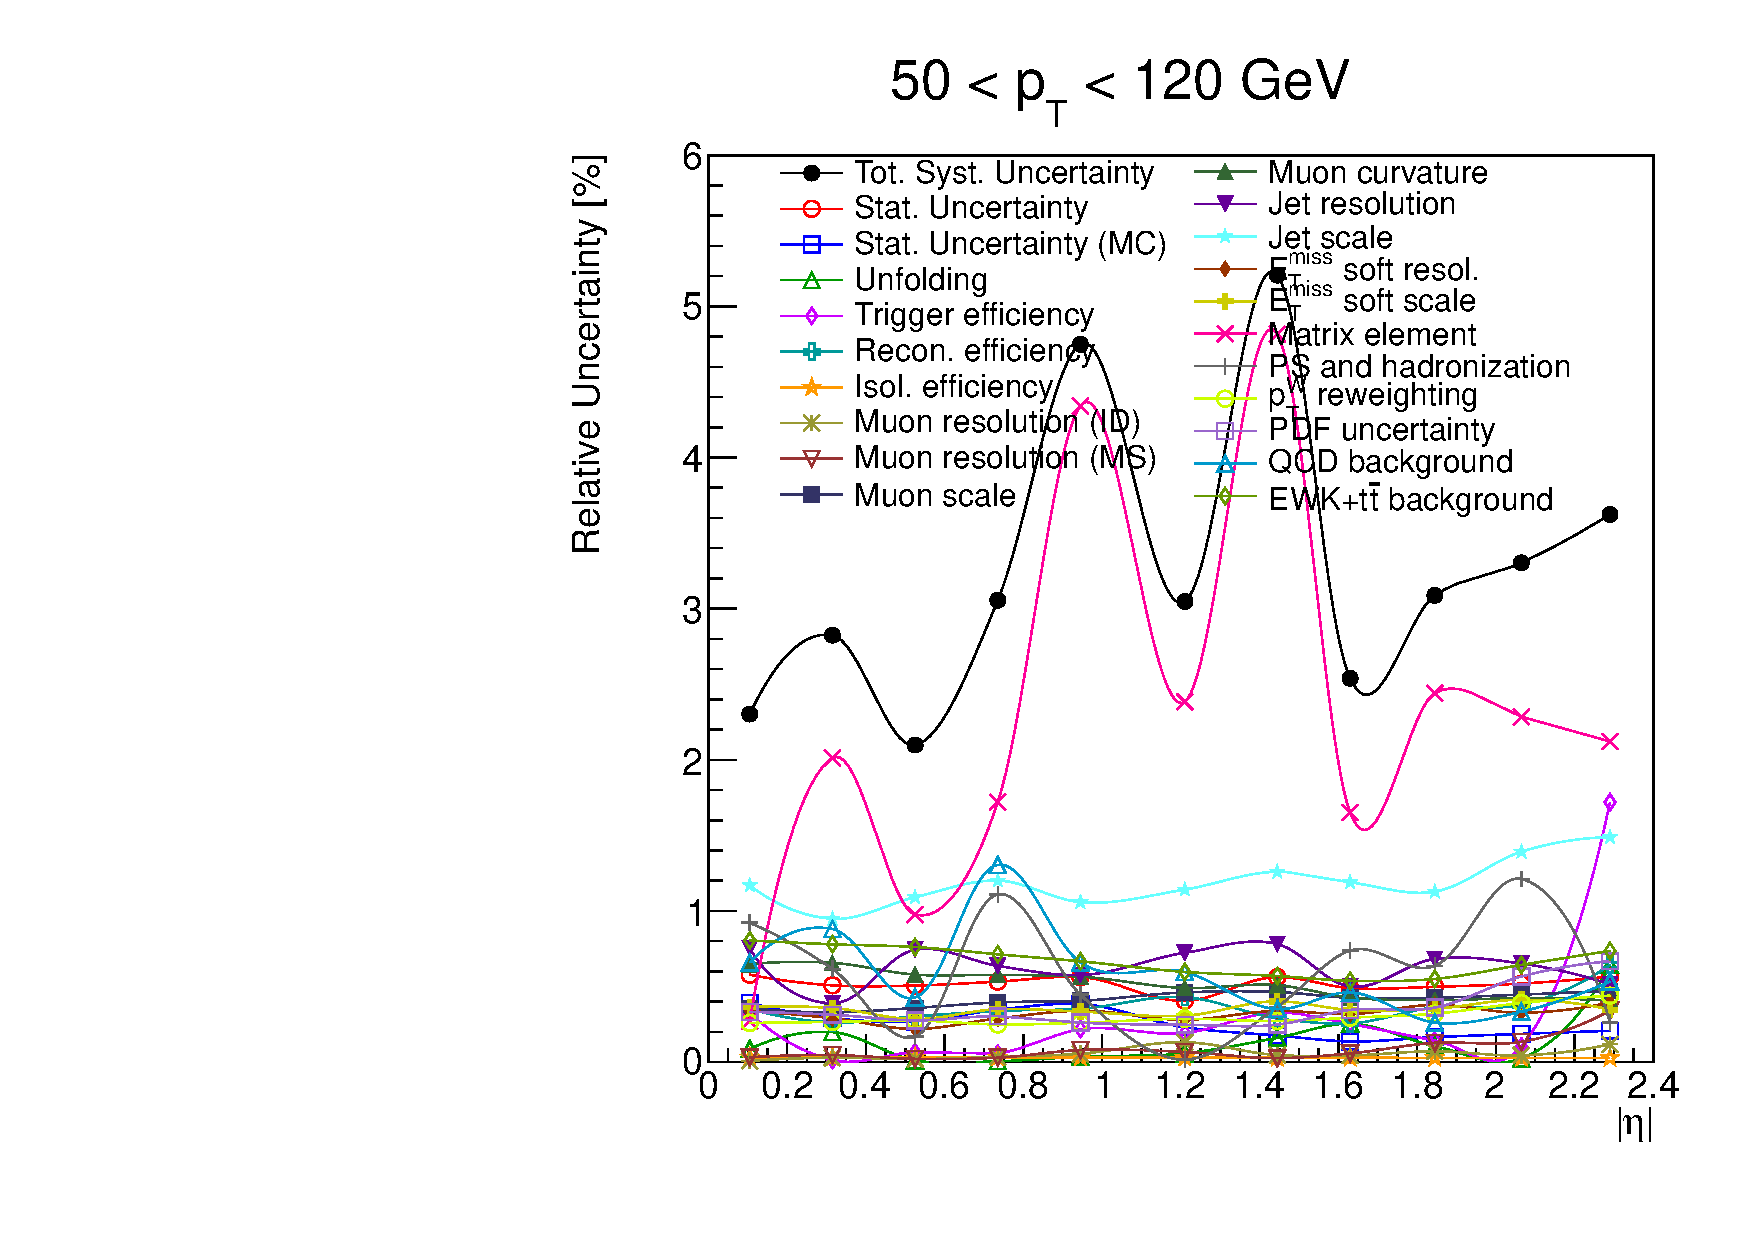
\includegraphics[width=0.3\textwidth]{dates/20121219/figures/xsec/NEG/Wmn_Unc_2d_Slice_7.pdf}
 \end{center}
\end{frame}


%%%%%%% Back-up slides %%%%%%%%%%
\appendix
\newcounter{finalframe}
\setcounter{finalframe}{\value{framenumber}}

\slide{}
{

\centering
\Huge Back-up slides
}
